
\section*{Appendix A: Mutual Fund Selection}
\par Our sample contains U.S. equity actively managed funds at the intersection of the CRSP Survivor-Bias-Free U.S. Mutual Fund database with the Thomson Reuters Mutual Fund Holdings S12 database. We use the MFLINKS database available from Wharton Research Data Services (WRDS) to combine both databases. Our final database contains mutual fund holdings spanning the period from January 2001 to December 2016. 
\subsection*{A.1 \hspace{0.1cm} CRSP Mutual Fund Database }
Since we wish to capture active mutual funds that invest primarily in U.S. equities, we follow \citet{kacperczyk2008unobserved} and  \citet{lou2012flow}, by eliminating balanced, bond, money market, international, index, and sector funds, as well as funds that do not primarily invest in U.S. common equity. We base our mutual fund selection on identifiers provided in the CRSP mutual fund database. Specifically, we select funds with the following Lipper Objective codes: ABR, B, CA, DL, EI, EMN, G, GI, I, LSE, MC, SG, SP. If a fund's Lipper Objective code is missing, we pick funds with the following Strategic Insight Objective codes:  AGG, GRI, GMC, GRO, ING, OPI, SCG. If both codes are missing for a fund, we select funds with the following Wiesenberger Fund Type codes: BAL, G, GCI, G-I, G-I-S, GS, G-S, G-S-I, I, IEQ, I-G, I-G-S, I-S, I-S-G, LTG, MCG, SCG, S-G-I, S-I, S-I-G.  
\par Since some funds misreport their objective code, we require funds to hold at least 80\% and at most 105\% in common stocks, on average. Index funds are eliminated based on the CRSP index fund flags (provided since 2003) and by screening fund names. In particular, funds are dropped if the fund name contains the following strings: INDEX, IND, INDX, IDX, IDX, MKT, MARKET, S&P, SP, MSCI, NYSE, RUSSELL, NASDAQ, ISHARES, DOWJONES, SPDR, ETF, 100, 400, 500, 600, 1000, 1500, 2000, 3000, 5000. Following \citet{kacperczyk2008unobserved}, to address the incubation bias\footnote{\citet{evans2004does} and \citet{kacperczyk2008unobserved} detect a form of survival bias in the CRSP mutual fund database, which stems from fund families sugarcoating their past performance. Fund families incubate private funds and only report the returns of the surviving incubated funds and do not disclose the past performance of terminated funds.} we delete observations for which the date of the observation is prior to the reported fund start-date and we delete observations with missing fund names. Other data from the CRSP mutual fund database include the total net assets (TNA), net returns (both monthly and daily), fees, and other qualitative fund data. We aggregate all different share classes belonging to a single fund at each point in time into one observation. Regarding the quantitative attributes of funds, we sum the TNA and we take a weighted average of the fund returns, expense ratio, turnover ratio and fees, using the lagged TNAs of each individual share class as weights. Regarding the qualitative attributes of funds (e.g., fund name, CRSP objective code, year of origin), the data of the oldest fund is retained. 

% The data on fund return is reported every month, while fund's TNA is reported on a quarterly/annual basis before 1992 and on a monthly basis after. Fund fees, such as expense ratio,  turnover ratio and 12(b)1 fees are reported annually before 1999 and quarterly after 1999.
\subsection*{A.2 \hspace{0.1cm} Thomson Reuters Database}
 Mutual fund holdings are provided by Thomson Reuters and are compiled from mandatory SEC fillings\footnote{Investment companies, which include mutual funds, insurance companies, banks, pension funds, and numerous other institutions are often called 13f institutions. These institutions are required to fill in a form with the Securities and Exchange Commission (SEC) on a semiannual basis.} and voluntary disclosures. From this database we exclude funds with the following objective codes: International, Municipal Bonds, Bond \& Preferred, Balanced and Metals. Every fund files the SEC form at the end of a quarter (the file date), which is often in the same quarter as the report date; the date for which the holdings are actually held (adjusted for stock splits\footnote{Adjustments are made using the cumulative adjustment factor for shares in the CRSP monthly file.}). To create a monthly time series of fund holdings, we keep reported holdings constant between report dates (e.g., holdings reported at the end of September are valid in October, November and December). A majority of funds report holdings on a quarterly basis, while a small number of funds have gaps between report dates of more than two quarters. To fill these gaps (of no more than two quarters), we impute holdings of missing quarters using the most recently available report date, assuming that these funds adopt a buy-and-hold strategy. In the final database about 65\% of the funds disclose their holdings quarterly, 34\% semi-annually, and 1\% on a less frequent basis.  


% A problem comes from late reporting or stale data, which reflects cases where the report and file date are not in the same quarter. There are cases of multiple file dates corresponding to the same report date (and the same holdings), which lead to gaps in holdings data. I delete all duplicate records of fund-report dates. 

% To obtain monthly funds holdings, I assume reported holdings are held in the subsequent months (no more than 3 months) up until the next report date (e.g., holdings reported at the end of September are valid for October, November and December).
\subsection*{A.3 \hspace{0.1cm} MFLINKS}
\par To combine the CRSP mutual fund database with the Thomson Reuters database, we use the MFLINKS provided by Russ Wermers on Wharton Research Data Services (WRDS). MFLINKS maps CRSP fund identifiers to Thomson Reuters fund identifiers, covering approximately 98\% of the domestic equity mutual funds. We manage to link about 92\% of the target universe in the CRSP mutual fund database to holdings data from Thomson Reuters. To ensure a reliable linkage between the two databases, we require that the TNAs reported by both databases do not differ by more than a factor of two. Finally, funds with less than 10 identified stock positions and less than \$5 million assets under management are excluded.  

% I manage to link 88.01\% of all fund-holdings observations to a CRSP stock by matching the CUSIP reported by Thomson Reuters with either the historic CUSIP (NCUSIP) or the header CUSIP (HCUSIP) reported in the CRSP monthly file. 
\par The final mutual fund database contains 2,871 distinct mutual funds including 92,903 fund-report dates and 314,362 fund-month observations. Table A1 presents the number of funds at the end of each year along with the TNA and number of holdings reported by Thomson Reuters. There is a rising trend in both the number of funds, the average fund size, and the market share held.

\begin{singlespacing}
\begin{table}[h!]
\centering
\small
\setlength{\tabcolsep}{14pt}
{\captionsetup{justification=centering,singlelinecheck=off}
\caption*{\bfseries Table A1: End of year summary statistics of the equity mutual fund sample} }
\caption*{This table presents summary statistics for the mutual fund database as of December each year. \textit{\#Holdings} is the number of reported holdings in Thomson Reuters. \textit{\#Distinct stocks} contains the number of unique stocks held by the funds in the sample and the aggregated percentage market share held. TNA is the total net assets under management reported by CRSP, expressed in millions USD.    } \label{tableA1} 
\begin{tabular}{llllllllllll}
\hline
Year & \#Funds & \multicolumn{2}{c}{\#Holdings} & \multicolumn{2}{c}{\#Distinct stocks} & \multicolumn{2}{c}{TNA(\$M)}  \\ \cline{3-8} 
     &           & Mean           & Median          & Mean            & \%Market           & Mean           & Median             \\ \hline
     2001 & 1,126 & 110    & 73 & 4,802 & 7.83  & 730.69  & 165.20 \\
2002 & 1,236 & 120 & 75 & 4,301 & 9.57  & 759.20  & 141.00 \\
2003 & 1,221 & 115 & 78 & 4,383 & 10.10 & 903.92  & 164.85 \\
2004 & 1,137 & 113 & 75 & 4,392 & 12.57 & 1,192.07 & 192.30 \\
2005 & 1,061 & 124 & 77 & 4,056 & 11.71 & 1,420.41 & 238.80 \\
2006 & 967  & 122 & 76 & 4,021 & 12.14 & 1,700.04 & 298.60 \\
2007 & 1,071 & 113 & 75 & 4,211 & 11.96 & 1,649.38 & 276.30 \\
2008 & 1,192 & 120 & 75 & 4,012 & 11.98 & 972.76  & 165.20 \\
2009 & 1,114 & 116 & 80 & 3,793 & 12.82 & 1,387.80 & 233.45 \\
2010 & 1,294 & 122 & 78 & 3,691 & 12.91 & 1,520.00 & 299.10 \\
2011 & 1,226 & 122 & 78 & 3,470 & 12.17 & 1,440.66 & 290.80 \\
2012 & 1,335 & 123 & 77 & 3,398 & 12.79 & 1,579.65 & 361.80 \\
2013 & 1,176 & 114 & 77 & 3,365 & 12.44 & 2,153.20 & 519.85 \\
2014 & 1,170 & 119 & 78 & 3,424 & 11.58 & 2,383.97 & 540.90 \\
2015 & 797  & 111 & 70 & 3,320 & 9.56  & 2,584.96 & 584.60 \\
2016 & 697  & 113 & 75 & 3,180 & 8.45  & 2,798.21 & 648.10
 \\ \hline   
\end{tabular}
\end{table}
\end{singlespacing}

\newpage 
\section*{Appendix B: Errors-in-variables (EIV) - corrected estimator}
The cross-sectional regression in Eq.(\ref{csr}) is inherently subject to the EIV bias, since the explanatory variables are estimations resulting from the first-pass time series regressions. Since $\hat{B}_{t-1}$ is estimated with error, the OLS-estimator of $\Gamma$ will be biased downwards. 
% \par Based on the works of \citet{theil1971principles} and \citet{litzenberger1979effect}, 
\par \citet{chordia2015cross} propose the following bias-corrected estimator of $\Gamma_t$ 
\begin{equation}
\label{shanken}
    \hat{\Gamma}^{EIV}_t = \left[\hat{X}'_{t-1}\hat{X}'_{t-1} - \sum^{N_t}_{i=1}M'\hat{\Sigma}_{\beta_{it-1}}M\right]^{-1}\hat{X}'_{t-1}R_t,
\end{equation}
where $\hat{X}_{t-1} = [\romannum{1}_{N_t} \hspace{0.1cm}\hat{B}_{t-1} \hspace{0.1cm} Z_{t-1}]$ contains the lagged regressors, $\romannum{1}_{N_t}$ is a $N_t$ $\times$ 1 vector of ones, $M$ is a $K$ $\times$ (1+$K$+$L$) matrix defined as $M$ = [$0_{K\text{x}1}$ $\romannum{1}_{K\text{x}K}$ $0_{K\text{x}L}$], and $\hat{
\Sigma}_{\beta_{it-1}}$ is the heteroskedasticity-consistent $K$ $\times$ $K$ covariance matrix estimator of \citet{white1980heteroskedasticity} for the estimation of the factor model parameters $\beta_{it-1}$. The matrix $M$ ensures that the bias-correction only affects the $K$ $\times$ $K$ submatrix $\hat{B}_{t-1}'\hat{B}_{t-1}$ of $X_{t-1}$. 
% \begin{equation}
%     \label{lambda}
%     \Lambda_t  = \begin{bmatrix} 0 & 0_{1\text{x}K} \\ 0_{K\text{x}1} & \sum_{i=1}^{N_t} \hat{\Sigma}_{\hat{\beta}^{t-1}_i} \end{bmatrix},
% \end{equation}
%  To allow for conditional heteroskedacity, we use the \citet{white1980heteroskedasticity} covariance matrix estimator for $\hat{\Sigma}_{\hat{\beta}^{t-1}_i}$. 
\par This bias-corrected estimator was originally proposed by \citet{theil1971principles} and \citet{litzenberger1979effect}. 
\citet{shanken1992estimation} generalize the EIV-corrected estimator and show that this estimator is consistent when $N_t$ diverges. \citet{chordia2015cross} gauge the statistical properties of the EIV-corrected estimator in simulations and show that the negative bias is reduced in comparison to the OLS estimator. \citet{raponi2017testing} employ this estimator in a small $T$ environment to test several prominent beta-pricing specifications of Fama-French using individual stocks. They find significant pricing ability of all factors, while the same risk premia often appear insignificantly different from zero when estimated using the traditional approach.  
\par The EIV-corrected estimator subtracts the estimated covariance matrix of the estimator of $\beta_{it}$ from $\hat{B}_{t-1}'\hat{B}_{t-1}$, to better approximate the true value of $B_{t-1}'B_{t-1}$. However, under a finite $T$ there is the possibility that this correction will overshoot, turning the matrix in parenthesis  nearly singular or even not positive definite. This may lead to extreme estimates of $\Gamma_t$ and nonsensical inference. 
\par To prevent this we apply the following procedure. Following \citet{chordia2015cross}, we reduce the likelihood of overshooting due to outliers by winsorizing each element of the estimated covariance matrix at the 5\% and 95\% levels across the cross-section of funds at each time $t$. Then, we apply the shrinkage procedure of \citet{raponi2017testing} using a shrinkage scalar $\lambda$ (0 $\leq$ $\lambda$ $\leq$ 1):
\begin{equation}
    \label{Y_EIV} 
    \hat{\Gamma}^{\text{EIV}}_{t} = \left[\hat{X}_{t-1}'\hat{X}_{t-1} - \lambda\sum^{N_t}_{i=1}M'\hat{\Sigma}_{\beta_{it-1}}M\right]^{-1}\hat{X}_{t-1}'R_{t}.
\end{equation}
When $\lambda$ is one we obtain the estimator in Eq.(\ref{shanken}), whereas when $\lambda$ is zero, we obtain the OLS estimator. The choice of shrinkage parameter $\lambda$ is dependent on the eigenvalues of the matrix in parenthesis. Starting from $\lambda$ = 1, if the minimum eigenvalue of this matrix is negative, we lower $\lambda$ by an arbitrary small amount set to 0.05. We also apply this shrinkage in case the difference between the EIV-corrected and OLS coefficients is bigger than 100\%. 
% \section*{Appendix B: Errors-in-variables (EIV) Bias}
% The estimation of risk premia is subjected to the EIV bias, because the set of regressors include estimations of factor betas. The OLS estimator for the factor betas for fund $i$ in month $t$ can be written as
% \begin{equation}
% \label{OLS_betas}
% \hat{\beta}_{it} = (F_{\tau,t}'F_{\tau,t})^{-1}F_{\tau,t}'R_{i\tau,t}, \hspace{0.2cm} \tau = t-\mathcal{T}+1,...,t. 
% \end{equation}
% The superscript $\tau$ is used to index the daily fund returns in the rolling window ending in month $t$ and $\mathcal{T}$ is the length of the rolling window, that is, two years ($\mathcal{T}$ $\approx$ 500 trading days). 
% The estimation error in the first stage is
% \begin{equation}
% \label{error}
%     u_{it} = \hat{\beta}_{it} - \beta_{it} = (F_{\tau,t}'F_{\tau,t})^{-1}F_{\tau,t}'\epsilon_{i\tau,t},  \hspace{0.2cm} \tau = t-\mathcal{T}+1,...,t. 
% \end{equation}
%  We stack the excess returns, factor betas estimates, residual returns, and estimation errors for all funds at each time $t$. Denote $R_s$ = [$R_{1s}$,...,$R_{N_ts}$]', $\hat{B}_t$ = [$\hat{\beta}_{1t}$,...,$\hat{\beta}_{N_tt}$]', $\epsilon_s$ = [$\epsilon_{1s},...,$\epsilon_{N_ts}$], and $U_t$ = [$u_{1t}$,...,$u_{N_tt}$]', given a total number of $N_t$ funds in the cross-section at time $t$. The second-pass regression in the Fama-MacBeth procedure is of the form $R_{s} = \hat{\gamma}_0 + \hat{B}_t\hat{\gamma} + \xi_s$, with time $s$ often simply one period ahead $t$+1. If we assume that the factor model holds ($\alpha$ = 0), the true model is $R_s = B_t\gamma + \epsilon_s$. The cross-sectional residuals are expressed as $\xi_s = (B_t - \hat{B}_t)\gamma + \epsilon_s$, which are correlated with the estimated factor betas. This endogeneity problem induces a downward bias in the estimated $\hat{\gamma}$. 
% \par Specifically, let $\romannum{1}_{N_t}$ be a $N_t$ $\times$ 1 column vector of ones and define $\hat{B}^*_t$ as [$\romannum{1}_{N_t}$ $\hat{B}_t$]. Then the OLS estimator of $\gamma$ is written as  

% \begin{equation}
%     \label{OLS}
%     \hat{\gamma}_{t+1} = (\hat{B}^*_t'\hat{B}^*_t)^{-1}\hat{B}^{*}_t R_{t+1}. 
% \end{equation}
% The expected value of the matrix in parenthesis is written as

% \begin{equation*}
%   E(\hat{B}^{*}_t'\hat{B}^{*}_t) = B^{*}_t'B^{*}_t+ \Lambda_t \hspace{0.2cm} \text{with} 
%   \end{equation*}
%   \begin{equation} 
%  \Lambda_t = \begin{bmatrix} 0 & 0_{1\times K} \\ 0_{K\times 1} & E(U_t'U_t) \end{bmatrix} =  \begin{bmatrix} 0 & 0_{1\times K} \\ 0_{K\times 1} & \sum_{i=1}^{N_t} E(u_{it}'u_{it}) \end{bmatrix} =  \begin{bmatrix} 0 & 0_{1\times K} \\ 0_{K\times 1} & \sum_{i=1}^{N_t} V(u_{it}') \end{bmatrix}.
% \end{equation}

% % \begin{equation}
    
% % \label{bias}
% % E(\hat{B}\romannum{1}_t'\hat{B}\romannum{1}_t) = B\romannum{1}_t'B\romannum{1}_t+ \Lambda_t, \hspace{0.1cm}  \text{with} \hspace{0.2cm}
% % \Lambda_t = \begin{bmatrix} 0 & 0_{1\text{x}K} \\ 0_{K\text{x}1} & E(U_t'U_t) \end{bmatrix} =  \begin{bmatrix} 0 & 0_{1\text{x}K} \\ 0_{K\text{x}1} & \sum_{i=1}^{N_t} E(U_{it}'U_{it}) \end{bmatrix} =  \begin{bmatrix} 0 & 0_{1\text{x}K} \\ 0_{k\text{x}1} & \sum_{i=1}^{N_t} V(U_{it}') \end{bmatrix}, 

% % \end{equation}
% Notice that the cross-products in the expectation of $\hat{B}^{*}_t'\hat{B}^{*}_t$ disappear as the estimate $\hat{B}_t$ is an unbiased estimator of $B_t$. The term V($u_{it}'$) is 
% \begin{equation}
% \label{white}
%     V(u_{it}') = E(u_{it}u_{it}')= (F_{\tau,t}'F_{\tau,t})^{-1}F_{\tau,t}'E(\epsilon_{i\tau,t}\epsilon_{i\tau,t}')F_{\tau,t}(F_{\tau,t}'F_{\tau,t})^{-1}, \hspace{0.2cm} \tau = t-\mathcal{T}+1,...,t, 
% \end{equation}
% which is simply the covariance matrix of the estimator of $\beta_{it}$, denoted by $\Sigma_{\beta_{it}}$.
% \par The right-bottom term of $\Lambda_t$ is the summation of covariance matrices of $N_t$ assets, which is positive semi-definite such that $\hat{B}^*_t'\hat{B}^{*}_t$ \textgreater $B^{*}_t'B^{*}_t$, leading to a negative bias in the estimated risk premia $\hat{\gamma}$. Notice that the second term in Eq.(\ref{OLS}), $\hat{B}^*_tR_t$ = $B^*_tR_t$ + $U_t'R_t$ does not systematically deviate from zero as $E(U_t'R_t)$ = 0.  The EIV bias is less severe when the estimation of $B_t$ is more precise. Assuming the true value of $B_t$ is time invariate, a way to improve precision is to increase the rolling window length $\mathcal{T}$. Asymptotically, the smaller measurement error in the first-pass regression reduces the bias in the second stage.
% \par A large stream of literature have followed \citet{jensen1972capital} and \citet{fama1973risk}, among many others, in mending the EIV bias by grouping assets into portfolios. The underlying motivation of grouping assets is to decrease idiosyncratic risk in the first-pass regression. Assuming unbiased estimates of the true factor betas and the estimation error being independent across different assets, the estimated factor betas of portfolios, which merely constitutes a weighted average of individual factor beta estimates, tend to become smaller as the portfolio contains a larger number of assets. Intuitively, the errors in estimated factor betas of individual assets tend to offset one another. Thus, creating portfolios allows for more efficient estimates of factor betas. 
% \par But using portfolios, rather than individual assets, has its own shortcomings. The number of test assets is dramatically reduced, such that there is less cross-sectional variation in factor betas to form risk premia estimates. Perhaps more alarming is that diversification into portfolios can mask cross-sectional phenomena in individual assets. \citet{liang2000portfolio} argue that measurement errors in the sorting variables can compound the EIV problem and further bias test results. \citet{ang2008using} show that the smaller standard errors of portfolio betas do not lead to smaller standard errors of the cross-sectional estimated risk premia.  
% \par Therefore, this paper will work with individual funds. This is in line with recent literature including the works of \citet{chordia2015cross}, \citet{jegadeesh2016empirical}, and \citet{raponi2017testing}. We employ the EIV-corrected estimator of \citet{chordia2015cross}, described in  Section 3.B.1.  
% \par \citet{pukthuanthong2014resolving} and \citet{jegadeesh2016empirical} have proposed an instrumental variables approach to mitigate the EIV bias. Recall that the explanatory variables in the second-pass regression suffer from endogeneity. A standard econometric solution is to define a particular set of well-behaved instruments which meet two conditions: (1) the instruments are correlated with the endogenous variables and (2) the instruments are uncorrelated with the residuals. They propose estimated factor betas from non-overlapping observations to serve as instruments for the second-pass regression. We have explored the IV estimator in simulations. The IV estimator did reduce the negative bias on $\gamma$, but exhibits the highest variability among all estimators.\footnote{In untabulated simulation results, the IV estimator ranked second behind the EIV-corrected estimator of \citet{chordia2015cross}. A major pitfall of instrumental variable estimation is the "weak instrument" problem, which is caused by low cross-correlations between endogenous variables and instruments, which may cause nonsensical estimates. Factor betas on value and momentum factors are most prone to time variation, due to the volatile nature of these anomalies. In simulations, these factors exhibit the highest variability due to low correlated instruments.}
% \newpage
% \section*{Appendix C: Simulation Experiments}
% In order to gauge the statistical properties of the proposed estimators of $\Gamma$ under small $T$ and large $N_t$, we resort to simulations with parameters matched to the real data. We investigate the bias and the root-mean-squared error (RMSE) of the OLS estimator and the EIV-corrected estimator. For this purpose a simple data-generating process is set, in which fund returns follow a six-factor model with time invariant factor betas:
% \begin{equation}
%     \label{carhart}
%     R_{it} = \beta_{i1} \text{RMRF}_t + \beta_{i2} \text{SMB}_t + \beta_{i3} \text{HML}_t + \beta_{i4} \text{WML}_t + \beta_{i5} \text{RMW}_t + \beta_{i6} \text{CMA}_t + \epsilon_{it}, 
% \end{equation}
% where $\text{RMRF}_t$ is the excess return on the market portfolio on day $t$. $\text{SMB}$, $\text{HML}$ and $\text{WML}$ are the factors from \citet{carhart1997persistence} and are excess returns on the factor mimicking portfolios for size (small minus big), book-to-market (high minus low) and one-year momentum (winners minus losers). The two additional factors RMW and CMA from \citet{FAMA20151} are factor returns for profitability (robust minus weak) and investment (conservative minus aggressive). The benchmark returns of RMRF, SMB, HML, WML, RMW and CMA are provided on Ken French's Website. 
% \par The simulation parameters are set equal to the corresponding parameters in the actual data covering the sample period of January 2001 to December 2016. For each fund, we estimate the six-factor model using rolling time series regressions based on  the past two years of daily return data. For the sake of simplicity, we assume the residuals are homoskedastic and compute the variance of residuals as $\hat{\sigma}_{\epsilon}^2$ = $\frac{\epsilon'\epsilon}{T-K}$. This results in a set of factor betas and residual variances from which we calculate the first two sample moments. 
% \par We conduct a simulation with 1000 replications where fund returns are randomly generated on a daily basis using the following procedure:
% \begin{enumerate}  
%     \item For each replication, we randomly generate daily factor returns for RMRF, SMB, HML, WML, RMW and CMA from normal distributions $\mathcal{N}$(0.025,1.520), $\mathcal{N}$(0.017,0.331), $\mathcal{N}$(0.014,0.398), $\mathcal{N}$(0.012,0.984), $\mathcal{N}$(0.019,0.200) and $\mathcal{N}$(0.013,0.131), respectively. These parameters are calculated using actual data on daily factor returns during our sample period. 
%     \item For each fund $i$, we randomly generate six-factor betas and $\hat{\sigma}_{\epsilon_i}$, which we keep constant over the entire sample period. The factor betas are generated from normal distributions $\mathcal{N}$(0.980,0.010), $\mathcal{N}$(0.197,0.114), $\mathcal{N}$(0.000,0.046), $\mathcal{N}$(0.021,0.015), $\mathcal{N}$(-0.057,0.043), and $\mathcal{N}$(-0.037,0,044). $\hat{\sigma}_{\epsilon_i}$ is generated from $\mathcal{N}$(0.293,0.031). All parameters are obtained from real data. 
%     \item For each fund $i$ and each day $t$, we randomly generate residual returns $\epsilon_{it}$ from independent normal distributions N(0,$\hat{\sigma}_{\epsilon_i}^2$).
% \end{enumerate}
% Then for each fund $i$ and each day $t$, we calculate the fund return according to Eq.(\ref{carhart}), using the realized factors (from step 1), the fund's factor betas (from step 2), and the residual return (from step 3). 
% \par We estimate the Fama-French six-factor model (first-stage regression) for each fund using a rolling window of the past two years of daily returns. The data is then aggregated to monthly frequency and the estimated betas are used in the second-stage cross-sectional regression (monthly fund returns on estimated factor betas) using the OLS and the EIV-corrected estimator. We roll the two-year estimation window forward by one month and repeat the risk premia estimation over the period February 2001 to December 2016, totalling 191 months. The final risk premia estimates are the time series averages of the $\hat{\gamma}_t$s. 
% \par We present the simulation results relative to the ex-ante risk premia (the true values) and also relative to the ex-post risk premia, which equal the time series means of the real factors and the simulated factor returns, respectively. \citet{shanken1992estimation} derive an expression for the ex-post risk premia as $\gamma^{ex-post}$ = $\gamma$ + $\bar{f}$ - E(f). As the true premium is the factor's expected value, the ex-post premium is simply the realized factor's sample mean. The notion of an ex-post premium is meaningful only conditional on the factor's realizations; as $T$ diverges, $\bar{f}$ will converge to E(f) and $\gamma^{ex-post}$ converges to the true value. However, under a finite $T$, $\gamma$ and $\gamma^{ex-post}$ will differ in general. The ex-post perspective is informative since it largely removes the component of estimation variance corresponding to factor outcomes, such that the performance of the EIV-correction relative to the residual variance component is highlighted. The ex-ante perspective presents the total picture, including factor surprises. Both the average bias and the average RMSE are reported from both perspectives.
% \par Table C1 reports the average bias and the average RMSE across 1000 replications, using $N$ $\in$ [250, 500, 1000, 2000] funds using a rolling window of the past two years to estimate factor betas.\footnote{In untabulated results, we find similar results when using rolling window sizes of one year, three years and five years. } Considering the bias relative to the ex-ante risk premia, the OLS estimations are, on average, always below the true risk premia, ranging from a negative bias between roughly 6\% for the size factor to a negative bias of roughly 23\% for the investment factor. This negative bias remains relatively stable when increasing the number of funds in the cross-section. The negative bias is similar when calculated relative to the ex-post risk premium. The negative bias is partially eliminated by the bias-corrected estimator, leading to a negative bias in the estimated risk premia ranging from 2\% to 7\%. 
% \par Next, we turn to the average RMSEs. Considering the ex-ante premia, the differences between the estimators are modest, almost equal for most factors. Recall that the RMSE is a function of both the bias and the variability of the estimator. Evidently, the OLS estimator has the smallest standard deviation, but it exhibits a more severe negative bias such that the RMSEs are similar. When considering the ex-post premia, there is a sharp reduction in RMSEs for both estimators, especially when correcting for the EIV bias. This indicates that a large part of the estimator's variability is caused by variability in factor outcomes. 
% \begin{singlespacing}

% \begin{table}[H]
% \small 
% {\captionsetup{justification=centering,singlelinecheck=off}
% \caption*{\bfseries Table C1: Simulation results }}
% \caption*{We simulate monthly fund returns from the a six-factor model: 
% $$ R_{it} = \beta_{i1} \text{RMRF}_t + \beta_{i2} \text{SMB}_t + \beta_{i3} \text{HML}_t + \beta_{i4} \text{WML}_t + \beta_{i5} \text{RMW}_t + \beta_{i6} \text{CMA}_t +  \epsilon_{it}.$$ At the beginning of each replication, we simulate daily factor returns from normal distributions with moments matched to sample moments from February 2001 to December 2016. Factor betas are drawn from normal distributions $\mathcal{N}$(0.980,0.010), $\mathcal{N}$(0.197,0.114), $\mathcal{N}$(0.000,0.046), N(0.021,0.015),  N(-0.057,0.043), and N(-0.037,0,044), respectively. We generate the residual variance $\hat{\sigma}_{\epsilon_i}$ from $\mathcal{N}$(0.293,0.031) and draw a residual return from N(0,$\hat{\sigma}^2_{\epsilon_i}$). For each fund $i$, factor betas are estimated from a rolling time series regression using the past two years of simulated daily fund returns. This table presents average biases and root-mean-squared errors (RMSEs) in risk premia estimated when the second stage regressions are fitted using the OLS and the EIV-corrected estimators, across 1000 replications. The bias and RSMEs are presented relative to the true risk premium (time series mean factor) and the ex-post risk premium of \citet{shanken1992estimation}. The latter is the time series average of factor returns in each replication.} 
% \centering
% \begin{tabular}{llllllllll}
% \hline
% Number & \multicolumn{4}{c}{Ex-ante premium}                 &  & \multicolumn{4}{c}{Ex-post premium}                 \\ \cline{2-5} \cline{7-10} 
% of     & \multicolumn{2}{c}{Bias} & \multicolumn{2}{c}{RMSE} &  & \multicolumn{2}{c}{Bias} & \multicolumn{2}{c}{RMSE} \\ \cline{2-5} \cline{7-10} 
% funds  & OLS         & EIV        & OLS         & EIV        &  & OLS         & EIV        & OLS         & EIV        \\ \hline
% \multicolumn{10}{l}{Panel A: \text{$\gamma_{MKT}$}}                                                                                  \\
% 250    & -0.095      & -0.025     & 0.214       & 0.215      &  & -0.100      & -0.029     & 0.114       & 0.051      \\
% 500    & -0.106      & -0.038     & 0.216       & 0.214      &  & -0.099      & -0.031     & 0.110       & 0.044      \\
% 1000   & -0.120      & -0.053     & 0.223       & 0.217      &  & -0.098      & -0.032     & 0.108       & 0.040      \\
% 2000   & -0.108      & -0.040     & 0.212       & 0.209      &  & -0.099      & -0.032     & 0.108       & 0.038      \\
%       &             &            &             &            &  &             &            &             &            \\
% \multicolumn{10}{l}{Panel B: \text{$\gamma_{SMB}$}}                                                                                  \\
% 250    & -0.012      & -0.007     & 0.138       & 0.145      &  & -0.008      & -0.002     & 0.022       & 0.017      \\
% 500    & -0.006      & 0.000      & 0.136       & 0.143      &  & -0.007      & -0.002     & 0.018       & 0.012      \\
% 1000   & -0.005      & 0.001      & 0.133       & 0.139      &  & -0.008      & -0.002     & 0.016       & 0.009      \\
% 2000   & -0.012      & -0.007     & 0.136       & 0.142      &  & -0.007      & -0.002     & 0.014       & 0.007      \\
%       &             &            &             &            &  &             &            &             &            \\
% \multicolumn{10}{l}{Panel C: \text{$\gamma_{HML}$}}                                                                                  \\
% 250    & -0.026      & -0.008     & 0.137       & 0.144      &  & -0.026      & -0.008     & 0.036       & 0.022      \\
% 500    & -0.022      & -0.004     & 0.134       & 0.141      &  & -0.026      & -0.008     & 0.033       & 0.017      \\
% 1000   & -0.028      & -0.011     & 0.126       & 0.132      &  & -0.025      & -0.007     & 0.030       & 0.013      \\
% 2000   & -0.024      & -0.006     & 0.132       & 0.138      &  & -0.026      & -0.008     & 0.030       & 0.012      \\
%       &             &            &             &            &  &             &            &             &            \\
% \multicolumn{10}{l}{Panel D: \text{$\gamma_{WML}$}}                                                                                  \\
% 250    & -0.199      & -0.061     & 0.272       & 0.220      &  & -0.198      & -0.060     & 0.207       & 0.077      \\
% 500    & -0.212      & -0.078     & 0.278       & 0.216      &  & -0.199      & -0.065     & 0.205       & 0.073      \\
% 1000   & -0.199      & -0.065     & 0.267       & 0.213      &  & -0.200      & -0.066     & 0.206       & 0.071      \\
% 2000   & -0.205      & -0.071     & 0.272       & 0.215      &  & -0.200      & -0.067     & 0.206       & 0.070      \\ \hline \end{tabular}
% \end{table}

% \begin{table}[H]
% \small
% \centering
% {\captionsetup{justification=centering,singlelinecheck=off}
% \caption*{\bfseries Table C1 (Continued)}}
% \begin{tabular}{llllllllll} \hline
% \multicolumn{10}{l}{Panel E: \text{$\gamma_{RMW}$}}                                                                            \\ 
% 250    & -0.054      & -0.013     & 0.116       & 0.116      &  & -0.057      & -0.017     & 0.065       & 0.029      \\
% 500    & -0.054      & -0.014     & 0.116       & 0.115      &  & -0.058      & -0.019     & 0.064       & 0.026      \\
% 1000   & -0.057      & -0.018     & 0.117       & 0.116      &  & -0.058      & -0.019     & 0.063       & 0.023      \\
% 2000   & -0.057      & -0.018     & 0.116       & 0.115      &  & -0.058      & -0.019     & 0.063       & 0.022      \\
%       &             &            &             &            &  &             &            &             &            \\
% \multicolumn{10}{l}{Panel F: \text{$\gamma_{CMA}$}}                                                                                  \\
% 250    & -0.051      & -0.020     & 0.097       & 0.094      &  & -0.044      & -0.014     & 0.050       & 0.024      \\
% 500    & -0.047      & -0.017     & 0.098       & 0.097      &  & -0.045      & -0.014     & 0.049       & 0.020      \\
% 1000   & -0.046      & -0.016     & 0.096       & 0.096      &  & -0.045      & -0.015     & 0.049       & 0.018      \\
% 2000   & -0.049      & -0.020     & 0.097       & 0.095      &  & -0.044      & -0.015     & 0.048       & 0.017      \\ \hline
% \end{tabular}
% \end{table}
% \end{singlespacing}

% \begin{singlespacing}
% \begin{table}[H]
% \small 
% {\captionsetup{justification=centering,singlelinecheck=off}
% \caption*{\bfseries Table C1: Simulation results }}
% \caption*{We simulate daily fund returns from the six-factor model: 
% $$ R_{it} = \beta_{i1} \text{RMRF}_t + \beta_{i2} \text{SMB}_t + \beta_{i3} \text{HML}_t + \beta_{i4} \text{WML}_t + \beta_{i5} \text{RMW}_t + \beta_{i6} \text{CMA}_t +  \epsilon_{it}.$$ At the beginning of each replication, we simulate daily factor returns from normal distributions with moments matched to sample moments from February 2001 to December 2016. Factor betas are drawn from normal distributions $\mathcal{N}$(0.980,0.010), $\mathcal{N}$(0.197,0.114), $\mathcal{N}$(0.000,0.046), N(0.021,0.015),  N(-0.057,0.043), and N(-0.037,0,044), respectively. We generate the residual variance $\hat{\sigma}_{\epsilon_i}$ from $\mathcal{N}$(0.293,0.031) and draw a residual return from N(0,$\hat{\sigma}^2_{\epsilon_i}$). For each fund $i$, factor betas are estimated from a rolling time series regression using the past two years of simulated daily fund returns. This table presents average biases and root-mean-squared errors (RMSEs) in risk premia estimated when the second stage regressions are fitted using the OLS and the EIV-corrected estimators, across 1000 replications. The bias and RSMEs are presented relative to the true risk premium (time series mean factor) and the ex-post risk premium of \citet{shanken1992estimation}. The latter is the time series averages of factor returns in each replication.} 
% \centering
% \label{my-label}
% \begin{tabular}{lrrrrrrrrr}
% \hline
% Number & \multicolumn{4}{c}{Ex-ante premium}                 &  & \multicolumn{4}{c}{Ex-post premium}                 \\ \cline{2-5} \cline{7-10} 
% of     & \multicolumn{2}{c}{Bias} & \multicolumn{2}{c}{RMSE} &  & \multicolumn{2}{c}{Bias} & \multicolumn{2}{c}{RMSE} \\ \cline{2-5} \cline{7-10} 
% funds  & OLS         & EIV        & OLS         & EIV        &  & OLS         & EIV        & OLS         & EIV        \\ \hline
% \multicolumn{10}{l}{Panel A: $\gamma_{RMRF}$}                                                                                 \\
% 250    & 0.013       & 0.062      & 0.421       & 0.470      &  & -0.048      & 0.001      & 0.226       & 0.240      \\
% 500    & -0.002      & 0.044      & 0.388       & 0.429      &  & -0.045      & 0.001      & 0.153       & 0.156      \\
% 1000   & 0.003       & 0.049      & 0.386       & 0.428      &  & -0.049      & -0.003     & 0.117       & 0.110      \\
% 2000   & 0.003       & 0.048      & 0.363       & 0.403      &  & -0.053      & -0.007     & 0.098       & 0.080      \\
%       &             &            &             &            &  &             &            &             &            \\
% \multicolumn{10}{l}{Panel B: $\gamma_{SMB}$}                                                                                  \\
% 250    & -0.029      & -0.016     & 0.185       & 0.191      &  & -0.012      & 0.001      & 0.065       & 0.066      \\
% 500    & -0.017      & -0.003     & 0.185       & 0.192      &  & -0.013      & 0.001      & 0.044       & 0.043      \\
% 1000   & -0.019      & -0.006     & 0.190       & 0.197      &  & -0.014      & 0.000      & 0.034       & 0.031      \\
% 2000   & -0.012      & 0.002      & 0.182       & 0.189      &  & -0.014      & 0.000      & 0.029       & 0.025      \\
%       &             &            &             &            &  &             &            &             &            \\
% \multicolumn{10}{l}{Panel C: $\gamma_{HML}$}                                                                                  \\
% 250    & -0.029      & -0.005     & 0.211       & 0.228      &  & -0.027      & -0.003     & 0.103       & 0.106      \\
% 500    & -0.035      & -0.012     & 0.207       & 0.222      &  & -0.023      & 0.000      & 0.073       & 0.074      \\
% 1000   & -0.022      & 0.002      & 0.196       & 0.211      &  & -0.022      & 0.002      & 0.058       & 0.054      \\
% 2000   & -0.012      & 0.013      & 0.188       & 0.204      &  & -0.024      & 0.000      & 0.046       & 0.038      \\
%       &             &            &             &            &  &             &            &             &            \\
% \multicolumn{10}{l}{Panel D: $\gamma_{WML}$}                                                                                  \\
% 250    & -0.032      & -0.007     & 0.340       & 0.377      &  & -0.020      & 0.005      & 0.172       & 0.185      \\
% 500    & -0.031      & -0.006     & 0.324       & 0.356      &  & -0.025      & 0.000      & 0.128       & 0.132      \\
% 1000   & -0.058      & -0.036     & 0.323       & 0.353      &  & -0.019      & 0.003      & 0.093       & 0.095      \\
% 2000   & -0.047      & -0.024     & 0.314       & 0.344      &  & -0.020      & 0.002      & 0.075       & 0.069           \\ \hline \end{tabular}
% \end{table}
% \end{singlespacing}
       
       
%  \begin{singlespacing}
%  \begin{table}[H]
% \small
% \centering
% {\captionsetup{justification=centering,singlelinecheck=off}
% \caption*{\bfseries Table C1 (Continued)}}
% \begin{tabular}{lrrrrrrrrr} \hline
% \multicolumn{10}{l}{Panel E: $\gamma_{RMW}$}                                                                                  \\
% 250    & -0.070      & -0.010     & 0.170       & 0.184      &  & -0.063      & -0.003     & 0.119       & 0.116      \\
% 500    & -0.067      & -0.006     & 0.150       & 0.158      &  & -0.064      & -0.004     & 0.096       & 0.079      \\
% 1000   & -0.067      & -0.007     & 0.152       & 0.161      &  & -0.064      & -0.004     & 0.085       & 0.059      \\
% 2000   & -0.071      & -0.013     & 0.149       & 0.154      &  & -0.064      & -0.006     & 0.077       & 0.042      \\
%       &             &            &             &            &  &             &            &             &            \\
% \multicolumn{10}{l}{Panel F: $\gamma_{CMA}$}                                                                                  \\
% 250    & -0.064      & -0.005     & 0.147       & 0.170      &  & -0.062      & -0.003     & 0.120       & 0.128      \\
% 500    & -0.066      & -0.008     & 0.135       & 0.150      &  & -0.062      & -0.004     & 0.101       & 0.094      \\
% 1000   & -0.063      & -0.006     & 0.123       & 0.134      &  & -0.065      & -0.007     & 0.086       & 0.063      \\
% 2000   & -0.065      & -0.009     & 0.120       & 0.127      &  & -0.066      & -0.009     & 0.080       & 0.044      \\ \hline
% \end{tabular}
% \end{table}
% \end{singlespacing}


\newpage
\section*{Appendix C: Probability Density Functions}

In this appendix several univariate and multivariate probability density functions are given which are used throughout this paper. For univariate densities, we indicate the first moment around the mean by $\mu$, whereas for multivariate densities this is indicated by $\pmb{\mu}}$.

        \subsection*{C.1 \hspace{0.1cm} Univariate Distributions} 
\textbf{Normal density:} \\ 
 The pdf of a normal distributed random variable $Z$ with mean $\mu$ and variance $\sigma^2$, that is, $Z$ $\sim$ $\mathcal{N}(\mu,\sigma^2 )$ is given by 
     \begin{equation} 
     p(Z|\mu,\sigma^2) = \frac{1}{\sqrt{2\pi\sigma^2}}\hspace{0.1cm} \text{exp}\left(-\frac{(Z-\mu)^2}{2\sigma^2}\right).
     \end{equation} 

\bigskip \newline
\noindent \textbf{Inverted Gamma-2 density:} \\
The pdf of an inverted Gamma-2 distributed random variable $Z$ with scale parameter $s$ $>$ 0 and degrees of freedom $v$ $>$ 0, that is, $Z$ $\sim$ $IG2(s,v)$ is given by 
     \begin{equation}
         p(Z|s,v) = c^{-1}Z^{-\frac{v+2}{2}} \text{exp}\left(-\frac{s}{2Z}\right),
     \end{equation}
     where $c$ = $\Gamma(v/2)\left(\frac{2}{s}\right)^{v/2}$. The mean and variance of Z are given by 
     \begin{equation*}
         E[Z] = \frac{s}{v-2} \hspace{2.2cm} \text{for} \hspace{0.1cm} v > 2
     \end{equation*}
      \begin{equation*}
         \text{Var}[Z] = \frac{2}{v-4} (E[Z])^2 \hspace{0.7cm} \text{for} \hspace{0.1cm} v > 4. 
     \end{equation*}
     \newpage
\subsection*{C.2 \hspace{0.1cm} Multivariate Distributions} 
\textbf{Multivariate Normal density:} \\ 
 The pdf of a multivariate normal distributed random variable $Z$ with k-dimensional location parameter $\pmb{\mu}$ and $k$ x $k$ positive definite symmetric covariance matrix $\Sigma$, that is, $Z$ $\sim$ $\mathcal{N}(\pmb{\mu},\Sigma )$ is given by 
     \begin{equation} 
     p(Z|\pmb{\mu},\Sigma) = \left(\frac{1}{\sqrt{2\pi}}\right)^k |\Sigma|^{-\frac{1}{2}} \text{exp}(-\frac{1}{2}(Z-\pmb{\mu})'\Sigma^{-1}(Z-\pmb{\mu})),  
     \end{equation} 
     where the mean and variance of $Z$ are $\pmb{\mu}$ and $\Sigma$, respectively.
\bigskip \newline 
\noindent  \textbf{Inverted Wishart density:}\\
The pdf of an inverted Wishart distributed $k$ x $k$ symmetric positive definite matrix $Z$ with degrees of freedom $v$ $\geq$ $k$ and symmetric positive definite scale matrix $S$, that is, $Z$ $\sim$ $IW(S,v)$ is given by 
     \begin{equation}
         p(Z|S,v) = c^{-1} \frac{|S|^{v/2}}{|Z|^{(v+k+1)/2}} \text{exp}\left(-\frac{1}{2}\text{tr}(Z^{-1}S)\right),
     \end{equation}
     where $c$ = $2^{\frac{vk}{2}}\Gamma_k\left(\frac{v}{2}\right)$.
     The mean of $Z$ is given by
      \begin{equation*}
         E[Z] = \frac{S}{v-k-1} \hspace{0.8cm} \text{for} \hspace{0.1cm} v > k + 1. 
     \end{equation*} 
     For a nice representation of the variance of Z, we refer to \citet{nydick2012wishart}. 


\newpage 

\newpage
\section*{Appendix D: Gibbs Sampler}


We provide the Gibbs sampler and the posterior distributions of the parameters in our model in Eqs.(\ref{asset}), (\ref{cross}) and (\ref{delta_t}), which we repeat here for convenience 
\begin{alignat}{2}
    R_{i\tau,t} &= \alpha_{it} + \beta_{it}'F_{\tau,t} + \epsilon_{i\tau,t}, \hspace{0.2cm} \epsilon_{i\tau,t} \sim \mathcal{N}(0,\sigma^2_{\epsilon_{it}}), \hspace{0.1cm} \tau = t-\mathcal{T}+1,...,t,
\hspace{0.1cm} i = 1,...,N_t \\
    \alpha_{it} &= \delta_{0t} + \delta_{1t}'Z_{it-1} + \eta_{it}, \hspace{0.2cm} \eta_{it} \sim \mathcal{N}(0,\sigma^2_{\eta t}), \hspace{0.1cm} t = 1,...,T, \\ 
    \delta_t &= \bar{\delta} + v_t, \hspace{0.2cm} v_t \sim \mathcal{N}(0,\Sigma_{\delta}), \hspace{0.1cm} t = 1,...,T.
\end{alignat}

For the sake of convenience, we can write the model in matrix form as 
\begin{alignat}{2}
    R_{i,t} &= X_tB_{it} + \epsilon_{i,t}  \\
    \alpha_{t} &= Y_{t-1}\delta_t + \eta_{t} \\ 
     \delta_t &= \bar{\delta} + v_t,
\end{alignat}
where $R_{i,t}$ is a $\mathcal{T}$ $\times$ 1 vector with daily returns of fund $i$ during the rolling window ending in month $t$, $X_t$ is a $\mathcal{T}$ $\times$ ($K$+1) matrix with a column of ones and the corresponding factor returns, $B_{it}$ = [$\alpha_{it}$, $\beta_{it}$]' contains the parameters of the factor model, and $\epsilon_{i,t}$ is a $\mathcal{T}$ $\times$ 1 vector with residuals. In the second equation, $\alpha_t$ is a $N_t$ $\times$ 1 vector with factor model alphas in month $t$, $Y_{t-1}$ is a $N_t$ $\times$ ($L$+1) matrix with a column of ones and the lagged fund-level characteristics for each fund, and $\eta_t$ is a $N_t$ $\times$ 1 vector with residuals. 

\subsection*{D.1 \hspace{0.1cm} Gibbs Sampler}
To initialize the Gibbs sampler, we require starting values for the model parameters. For the fund-specific parameters, we estimate Eq.(\ref{asset}) for each fund in each rolling window and use the estimates as starting values for $\alpha_{it}$ and $\beta_{it}$. Each month $t$, we regress the estimates of alpha on a constant and the lagged characteristics using the cross-section of funds. The resulting estimates are used as starting values for $\delta_t$. The starting values for $\sigma^2_{\epsilon_{it}}$ and $\sigma^2_{\eta t}$ are set to the sample residual variance estimator from the corresponding regressions. For the hyperparameters $\bar{\delta}$ and $\Sigma_\delta$, we set the starting values equal to the sample mean and covariance matrix of the estimates $\{\delta_t\}^T_{t=1}$, respectively. The Gibbs sampler uses an iterative procedure to create Markov chains by simulating from full conditional posteriors. The algorithm below summarizes the steps in the Gibbs sampler.

\renewcommand\labelenumi{\theenumi:}
\begin{algorithm}
\caption{MCMC Gibbs sampler}\label{gibbs}
 \textsc{Inputs}: \{\{\{$R_{i\tau,t}, Z_{it-1}, F_{\tau,t}\}_{i=1} ^{N_t}}\}_{\tau = t -\mathcal{T} +1}^{t}\}_{t=1}^{T}$ (data)\\
\textsc{Outputs}: $\{\theta^{(m)}\}_{m=1}^{M}$ (approximate sample from the joint posterior)  \vspace{0.2cm} \hline 
 \begin{minipage}{.92\linewidth}
 \vspace{0.2cm}
\begin{enumerate}
\item Set starting values for model parameters: \\ $\theta^{(0)}$ =  $\{ \{\{\alpha_{it}^{(0)}, \beta_{it}^{(0)}, \sigma^2_{\epsilon_{it}}^{(0)}\}^{N_t}_{i=1}, \delta^{(0)}_{t}, \sigma^2_{\eta t}^{(0)}\}^{T}_{t=1}, \bar{\delta}^{(0)}, \Sigma^{(0)}_{\delta}\}$ and set $m$ to 0. 
\item Update parameters given current draws $\theta^{(m)}$:
\begin{enumerate}[label=(\roman*)]
    \item Sample $\alpha_{it}^{(m+1)}$, $\beta_{it}^{(m+1)}$ $|$ $\sigma^2_{
 \epsilon_{it}}^{(m)}$, $\delta_t^{(m)}$, 
  $\sigma^2_{\eta t}^{(m)}$, \hspace{0.1} for $i$ = 1,...,$N_t$, $t$ = 1,...,$T$. 
  \item Sample $\sigma^2_{\epsilon_{it}}^{(m+1)}$ $|$ $\alpha^{(m+1)}_{it}$, $\beta_{it}^{(m+1)}$, \hspace{0.1} for $i$ = 1,...,$N_t$, $t$ = 1,...,$T$. 
    \item Sample $\delta_{t}^{(m+1)}$ $|$ $\{\alpha_{it}^{(m)}\}^{N_t}_{i=1}$, $\sigma^2_{\eta t}^{(m)}$, $\bar{\delta}^{(m)}$, $\Sigma_{\delta}^{(m)}$, \hspace{0.1} for $t$ = 1,...,$T$. 
    \item Sample $\sigma^2_{\eta t}^{(m+1)}$ $|$ $\{\alpha_{it}^{(m+1)}\}^{N_t}_{i=1}$, $\delta^{(m+1)}_t$, \hspace{0.1} for $t$ = 1,...,$T$.
    \item Sample $\bar{\delta}^{(m+1)}$ $|$ $\{\delta_t^{(m+1)}\}^{T}_{t=1}$, $\Sigma_{\delta}^{(m)}$. 
    \item Sample $\Sigma_{\delta}^{(m+1)}$ $|$ $\{\delta_t^{(m+1)}\}^{T}_{t=1}$, $\bar{\delta}^{(m+1)}$. 
\end{enumerate}
\item Set $m$ = $m$ + 1, and go to step 2. 
\end{enumerate} 
\end{minipage}
\end{algorithm}
\newpage

 \subsection*{D.2 \hspace{0.1cm} Joint Posterior Distribution}
The joint posterior distribution is proportional to the product of the likelihood function of the data and the prior distributions. Denote $\theta$ =  $\{ \{\{\alpha_{it}, \beta_{it}, \sigma^2_{\epsilon_{it}}\}^{N_t}_{i=1}, \delta_{t}, \sigma^{2}_{\eta t}\}^{T}_{t=1}, \bar{\delta}, \Sigma_{\delta}\}$ as the model parameters. Denote $R$ as the matrix which stacks the returns in the rolling windows across all funds over the entire sample period. Substituting the prior specifications as in Section \ref{priors}, the joint posterior is given by: 
\begin{alignat}{2}
\label{joint}
p(\theta|R) &\propto p(R|\theta)p(\theta) \nonumber \\  
 &\propto \prod^T_{t=1} \prod^{N_t}_{i=1} \hspace{0.1cm} (\sigma^2_{\epsilon_{it}})^{-\frac{\mathcal{T}}{2}} \hspace{0.1cm} \text{exp}\left[-\frac{1}{2\sigma^2_{\epsilon_{it}}}(R_i- X_tB_{it})' (R_i- X_tB_{it})\right]  \nonumber \\  
      &\times \prod^{T}_{t=1} \hspace{0.1cm} (\sigma^2_{\eta t})^{-\frac{N_t}{2}}\hspace{0.1cm} \text{exp}\left[-\frac{1}{2\sigma^2_{\eta t}}(\alpha_t- Y_{t-1}\delta_{t})'(\alpha_t- Y_{t-1}\delta_{t})\right]  \nonumber \\  
      &\times \prod^{T}_{t=1} \prod^{N_t}_{i=1} \hspace{0.1cm}|\Sigma_{\beta}|^{-\frac{1}{2}}\hspace{0.1cm}\text{exp}\left[-\frac{1}{2}(\beta_{it}-\bar{\beta})'\Sigma^{-1}_{\beta}(\beta_{it}-\bar{\beta})\right]   \nonumber \\  
  &\times \prod^{T}_{t=1} \hspace{0.1cm} |\Sigma_{\delta}|^{-\frac{1}{2}} \hspace{0.1cm} \text{exp}\left[-\frac{1}{2}(\delta_{t}-\bar{\delta})'\Sigma^{-1}_{\delta} (\delta_{t}-\bar{\delta})\right] \nonumber \\  
  &\times |\Sigma_d|^{-\frac{1}{2}} \hspace{0.1cm} \text{exp}\left[-\frac{1}{2}(\bar{\delta} - d)'\Sigma^{-1}_d (\bar{\delta} - d) \right]  \nonumber \\  
  &\times |\Sigma_{\delta}|^{-\frac{\psi_\delta + k + 1}{2}} \hspace{0.1cm} \text{exp}\left[-\frac{1}{2} \text{tr}(\Sigma^{-1}_{\delta} [\psi_\delta S_\delta])\right] \nonumber \\  
  &\times \prod^{T}_{t=1}\prod^{N_t}_{i=1} \hspace{0.1cm} \sigma_{\epsilon_{it}}^{(v_\epsilon+2)}\hspace{0.1cm}\text{exp}\left(-\frac{s_\epsilon}{2\sigma^2_{\epsilon_{it}}}\right) \nonumber \\  
  &\times \prod^{T}_{t=1}\hspace{0.1cm}\sigma_{\eta t}^{(v_\eta + 2)}\hspace{0.1cm}\text{exp}\left(-\frac{s_\eta}{2\sigma^2_{\eta t}}\right),
\end{alignat} 
where $k$ denotes the dimension of $\Sigma_\delta$. 
 
 \subsection*{D.3 \hspace{0.1cm} Conditional Posterior Distributions}
In order to implement the MCMC Gibbs sampler, we need to derive the full conditional posterior distributions for each block of model parameters. The conditional densities can be obtained from the joint posterior density by gathering all the terms that depend on the parameters of interest and ignore all the remaining parameters. We then obtain the conditional density for each block of parameters by rearranging the remaining terms into the kernel of a known distribution.\footnote{Appendix D provides the probability density functions (pdfs) of the distributions used in our analysis.} We partition the model parameters $\theta$ into the following blocks: 
\begin{itemize}
    \item $\theta^{(1)}$: Fund-specific factor model parameters ($\alpha_{it}$, $\beta_{it}$)
    \item $\theta^{(2)}$: Fund-specific idiosyncratic variance ($\sigma^2_{\epsilon_{it}}$)
    \item $\theta^{(3)}$:  Characteristic loadings ($\delta_{0t}$, $\delta_{1t}$)
    \item $\theta^{(4)}$: Cross-sectional idiosyncratic variance ($\sigma^2_{\eta t}$)
        \item $\theta^{(5)}$: Time series mean of characteristic loadings ($\bar{\delta}$)
    \item $\theta^{(6)}$: Time series covariance matrix of  characteristic loadings ($\Sigma_{\delta}$)

\end{itemize}
\par The conditional posteriors for all parameters have convenient functional forms which trace back to a known distribution. Therefore, we use the Gibbs sampler to iteratively draw from the full conditional distributions of $\theta^{(1)}$, $\theta^{(2)}$, $\theta^{(3)}$, $\theta^{(4)}$, $\theta^{(5)}$, and $\theta^{(6)}$. Using the joint posterior distribution in Eq.(\ref{joint}), we will derive the full conditional posteriors for each block. 

\subsection*{D.3.1 \hspace{0.1cm} Conditional Posterior [$\alpha_{it}$ $\beta_{it}$]'} 
 In order to derive the full conditional posterior of [$\alpha_{it}$ $\beta_{it}$]', we require the following mathematical relations.
First, we require
\begin{equation}
\label{choleski}
B^{-1} = B^{-\frac{1}{2}}' B^{-\frac{1}{2}},
\end{equation}
 which is denoted the Cholesky decomposition, i.e., the decomposition of a positive-definite matrix into the product of a lower triangular matrix and its conjugate transpose. We also require the decomposition rule:
 \begin{equation}
     \label{decompostion}
     (y-X\beta)'(y-X\beta) = (y-X\hat{\beta})'(y-X\hat{\beta})+ (\beta-\hat{\beta})'X'X(\beta-\hat{\beta}),
 \end{equation}
 where $\hat{\beta}$ = $(X'X)^{-1}X'y$ is the OLS estimator of $\beta$.
 \par Following Bayes' theorem, we can write
\begin{alignat}{2}
p(B_{it}|R) &\propto p(R|B_{it})p(B_{it})  \nonumber  \\ 
 &\propto  \text{exp}\left[-\frac{1}{2\sigma^2_{\epsilon_{it}}}(R_{i,t}-X_tB_{it})'(R_{i,t}-X_tB_{it})\right] \times \text{exp}\left[-\frac{1}{2}(B_{it}-\bar{B}_{it})'\Sigma^{-1}_{B_{it}}(B_{it}-\bar{B}_{it})\right],  \nonumber  \\ & \text{where} \hspace{0.1cm} \bar{B}_{it} = \begin{bmatrix} \delta_{0t} + \delta'_{1t}Z_{it-1} \\ \bar{\beta} \end{bmatrix} \hspace{0.1cm} \text{and} \hspace{0.2cm} \Sigma_{B_{it}} = \begin{bmatrix} \sigma^2_{\eta t} & 0_{1\times K} \\ 0_{K \times 1} & \Sigma_{\beta} \end{bmatrix} \nonumber  \\ 
      &= \text{exp}\left[-\frac{1}{2}\left( \frac{1}{\sigma^2_{\epsilon_{it}}} (R_{i,t}-X_tB_{it})'(R_{i,t}-X_tB_{it}) + (\Sigma^{-\frac{1}{2}}_{B_{it}}\bar{B}_{it} - \Sigma^{-\frac{1}{2}}_{B_{it}}B_{it})'(\Sigma^{-\frac{1}{2}}_{B_{it}}\bar{B}_{it} - \Sigma^{-\frac{1}{2}}_{B_{it}}B_{it})\right)\right] \nonumber  \\ 
& \text{using} \hspace{0.1cm} \text{Eq.(\ref{choleski})} \nonumber  \\ 
  &= \text{exp} \left[-\frac{1}{2}(w_{it}-V_{it}B_{it})'(w_{it}-V_{it}B_{it})\right], \nonumber \\ 
  & \text{where} \hspace{0.1cm} w_{it} = \left[\sigma^{-1}_{\epsilon_{it}}R_{i,t} \hspace{0.25cm} \Sigma^{-\frac{1}{2}}_{B_{it}} \bar{B}_{it} \right]' \hspace{0.1cm} \text{and} \hspace{0.1cm} V_{it} =  \left[\sigma^{-1}_{\epsilon_{it}} X_t \hspace{0.25cm} \Sigma^{-\frac{1}{2}}_{B_{it}} \right]' \nonumber \\ 
  &\propto  \text{exp}\left[(B_{it} - \hat{B}_{it})'V_{it}'V_{it}(B_{it} - \hat{B}_{it})\right], \hspace{0.1cm} \text{using} \hspace{0.1cm} \text{Eq.}(\text{\ref{decompostion}}), \nonumber \\ 
  & \text{where} \hspace{0.1cm} \hat{B}_{it} = (V_{it}'V_{it})^{-1}V_{it}'w_{it},
\end{alignat}  
\noindent which is the kernel of a normal distribution with mean  $\hat{B}_{it}$ and variance $(V_{it}'V_{it})^{-1}$, that is, 
the full conditional posterior\footnote{Let $\theta^{-(x)}$ denote the model parameters excluding the set $x$.} of $B_{it}$ = [$\alpha_{it}$ $\beta_{it}$]' follows a multivariate normal distribution and is given by 
\begin{equation}
    \begin{bmatrix} \alpha_{it} \\ \beta_{it} \end{bmatrix} | \theta^{-(\alpha_{it}, \beta_{it})},R \sim \mathcal{N}\left(\tilde{B}_{it},\left[\sigma^{-2}_{\epsilon_{it}}X_{t}'X_t + \Sigma^{-1}_{B_{it}}\right]^{-1}}\right),
\end{equation}
with 
\begin{equation}
    \tilde{B}_{it} = \left[\sigma^{-2}_{\epsilon_{it}}X_{t}'X_t + \Sigma^{-1}_{B_{it}}\right]^{-1}\left[\sigma^{-2}_{\epsilon_{it}}X'_tR_t + \Sigma^{-1}_{B_{it}}\bar{B}_{it}\right].
\end{equation}
% with
% \begin{equation}
% \tilde{B}_{i,t} = \left[\sigma^{-2}_{\epsilon_{it}}X_t'X_t + \Sigma^{-1}_{B_{i,t}}\right]^{-1}\left[\sigma^{-2}_{\epsilon_{it}} X_t'R_{i,t}+ \Sigma^{-1}_{B_{i,t}}\bar{B}_{i,t}\right], 
% \end{equation}
% where $R_{i,t}$ is a $\mathcal{T}$ $\times$ $1$ vector with the returns of fund $i$ in the rolling window period ending at month $t$, $F_t$ is a $\mathcal{T}$ $\times$ ($K+1$) matrix in which the first column is a vector of ones and the remaining columns contain the returns of the $K$ factors over the same period. 
% Parameters $\bar{\lambda}_{i,t}$ and $\Sigma_{\lambda_{i,t}}$ are defined as 
% \begin{align} 
% \bar{\lambda}_{i,t} = \begin{bmatrix} X_{i,t}\delta_t \\ \bar{\beta} \end{bmatrix} && \Sigma_{\lambda_{i,t}} = \begin{bmatrix} \sigma^2_{\eta t} & 0_{1\times K} \\ 0_{K \times 1} & \Sigma_{\beta} \end{bmatrix}.
% \end{align} 
 We derive the full conditional posteriors of $\delta_{t}$ and  $\bar{\delta}$ in the same way, leading to the following results.
 
 \subsection*{D.3.2 \hspace{0.1cm} Conditional Posterior $\delta_t$}
The full conditional posterior of $\delta_t$ follows a multivariate normal distribution and is given by 
\begin{equation}
     \delta_t | \theta^{-(\delta_{t})},R \sim \mathcal{N}\left(\tilde{\delta}_t,\left[\sigma^{-2}_{\eta t}Y_{t-1}'Y_{t-1} + \Sigma^{-1}_{\delta}\right]^{-1}}\right),
\end{equation}
with
\begin{equation}
\tilde{\delta}_{t} = \left[\sigma^{-2}_{\eta t}Y_{t-1}'Y_{t-1} + \Sigma^{-1}_{\delta}\right]^{-1}\left[\sigma^{-2}_{\eta t}Y_{t-1}'\alpha_{t}+ \Sigma^{-1}_{\delta}\bar{\delta}\right].
\end{equation}

\subsection*{D.3.3 \hspace{0.1cm} Conditional Posterior $\bar{\delta}$}
The full conditional posterior of $\bar{\delta}$ follows a multivariate normal distribution and is given by 
\begin{equation}
     \bar{\delta}| \theta^{-(\bar{\delta})},R \sim \mathcal{N}\left(\tilde{\bar{\delta}},\left[T\Sigma^{-1}_{\delta} +\Sigma^{-1}_d}\right]^{-1}}\right),
\end{equation}
with
\begin{equation}
\tilde{\bar{\delta}} = \left[T\Sigma^{-1}_{\delta} +\Sigma^{-1}_d}\right]^{-1}\left[\Sigma^{-1}_{\delta} \sum_{t=1}^T \delta_t + \Sigma^{-1}_{d}d\right]. 
\end{equation}

\newpage
\subsection*{D.3.4 \hspace{0.1cm} Conditional Posterior $\Sigma_{\delta}$}
In order to derive the full conditional posterior of $\Sigma_{\delta}$, we require the following mathematical relations. First, we require
\begin{align}
\label{scalar}
    A &= \text{tr}(A) \\ 
      \label{perm}
        \text{tr}(ABC) &= \text{tr}(CAB) = \text{tr}(BCA) \\
        \label{sum}
 \text{tr}(A) + \text{tr}(B) &= \text{tr}(A+B),
    \end{align}
    where tr denotes the trace of a matrix. The above relations state that the trace of a scalar is equivalent to the scalar itself, that the trace is invariant under cyclic permutations, and that the sum of traces equals the trace of the sum. 
\par Following Bayes' theorem, we can write 
\begin{alignat}{2}
p(\Sigma_{\delta}|R) &\propto  p(\Sigma_{\delta})p(\delta_t)  \nonumber  \\
 &\propto |\Sigma_{\delta}|^{-\frac{\psi_{\delta} + k + 1}{2}}  \text{exp}\left[-\frac{1}{2}\text{tr}(\Sigma^{-1}_{\delta} [\psi_{\delta}S_{\delta}])\right] \times \prod^{T}_{t=1} \hspace{0.1cm} |\Sigma_{\delta}|^{-\frac{1}{2}}  \text{exp}\left(-\frac{1}{2}(\delta_{t} - \bar{\delta})' \Sigma^{-1}_{\delta}(\delta_{t} - \bar{\delta})\right) \nonumber  \\ 
      &= 
      |\Sigma_{\delta}|^{-\frac{\psi_{\delta} + T + k + 1}{2}} \text{exp}\left[-\frac{1}{2}\left(\text{tr}(\Sigma^{-1}_{\delta} [\psi_{\delta}S_{\delta}]) + \text{tr}\left(\sum^{T}_{t=1}(\delta_{t} - \bar{\delta})' \Sigma^{-1}_{\delta}(\delta_{t} - \bar{\delta}) \right)\right) \right], \   \nonumber  \\ 
      & \text{using} \hspace{0.1cm} \text{Eq.}(\text{\ref{scalar}}) \nonumber \\ 
&= 
      |\Sigma_{\delta}|^{-\frac{\psi_{\delta} + T +k + 1}{2}} \text{exp}\left[-\frac{1}{2}\left(\text{tr}(\Sigma^{-1}_{\delta} [\psi_{\delta}S_{\delta}]) + \text{tr}\left(\sum^{T}_{t=1}\Sigma^{-1}_{\delta}(\delta_{t} - \bar{\delta})(\delta_{t} - \bar{\delta})' \right) \right)\right],  \nonumber  \\ 
         & \text{using} \hspace{0.1cm} \text{Eq.}(\text{\ref{perm}}) \nonumber \\ 
&= 
      |\Sigma_{\delta}|^{-\frac{\psi_{\delta} + T + k + 1}{2}} \text{exp}\left[-\frac{1}{2}\text{tr}\left(\Sigma^{-1}_{\delta} \left[\sum^{T}_{t=1}(\delta_{t} - \bar{\delta}) (\delta_{t} - \bar{\delta})' +  \psi_{\delta}S_{\delta} \right]\right)\right], \nonumber  \\ 
            & \text{using} \hspace{0.1cm} \text{Eq.}(\text{\ref{sum}}),
\end{alignat} 
which is the kernel of an inverted Wishart distribution, that is, the full conditional posterior distribution of $\Sigma_{\delta}$ is given by

    \begin{equation}
    \Sigma_{\delta}|\theta^{(-\Sigma_{\delta})},R \sim \mathit{IW}\left(\sum^{T}_{t=1}(\delta_{t}-\bar{\delta})(\delta_{t}-\bar{\delta})'+\psi_{\delta}S_{\delta},\psi_{\delta} + T\right).
\end{equation}

\subsection*{D.3.5 \hspace{0.1cm} Conditional Posterior $\sigma^2_{\epsilon_{it}}$}
Following Bayes' theorem, we can write
\begin{alignat}{2}
p(\sigma^2_{\epsilon_{it}}|R) &\propto p(R|\sigma^2_{\epsilon_{it}})p(\sigma^2_{\epsilon_{it}})  \nonumber  \\
 &\propto \sigma^{-(\mathcal{T}+v_\epsilon + 2)}_{\epsilon_{it}}  \text{exp}\left[-\frac{1}{2\sigma^2_{\epsilon_{it}}}\left((R_{i,t} - X_tB_{it})'(R_{i,t} - X_tB_{it}) + s_\epsilon\right)\right], 
\end{alignat} 
which is the kernel of an inverted Gamma-2 distribution, that is, the full conditional posterior distribution of $\sigma^2_{\epsilon_{it}}$ is given by 
\begin{equation}
    \sigma^2_{\epsilon_{it}}|\theta^{(-\sigma^2_{\epsilon_{it}})},R \sim \mathit{IG}2\left((R_{i,t} - X_tB_{it})'(R_{i,t} - X_tB_{it}) + s_\epsilon,\mathcal{T} + v_\epsilon \right).
\end{equation}

\subsection*{D.3.6 \hspace{0.1cm} Conditional Posterior $\sigma^2_{\eta t}$}
The full conditional posterior of $\sigma^2_{\eta t}$ follows an Inverted Gamma-2 distribution and is given by 
\begin{equation}
    \sigma^2_{\eta t}|\theta^{(-\sigma^2_{\eta t})},R \sim \mathit{IG}2\left((\alpha_{t} - Y_{t-1}\delta_{t})'(\alpha_{t} -  Y_{t-1}\delta_{t}) + s_\eta, N_t + v_\eta \right). 
\end{equation}

\newpage
\subsection*{Appendix E: Construction of Benchmark Portfolios of DGTW Characteristic Selectivity Measure}
We construct the benchmark portfolios in the spirit of Daniel, Grinblatt, Titman, and Wermers (DGTW; 1997). We proceed as follows. We conduct a three-dimensional sort along the size, value and momentum dimensions. All stocks having accounting data from Compustat, as well stock return and market capitalization data are sorted into quintile portfolios by their market capitalization. The breakpoints for the sort on size is based on stocks listed on the NYSE, while the analysis includes all stocks listed on the NYSE, NYSE MKT (formerly known as AMEX), and NASDAQ. Each size quintile is further subdivided into quintiles based on the book-to-market ratio of stocks, resulting into 25 fractile portfolios. Then, each fractile portfolio is further subdivided into quintiles based on the past twelve-month cumulative return excluding the most recent month. This 5x5x5 sorting procedure leads to 125 portfolios, each with a unique combination of size, value, and momentum rankings.\footnote{For example, a stock sorted in size portfolio five, value portfolio five, and momentum five, is a large, value and high momentum stock.} 
\par Next, to adjust for profitability and investment effects, we also conduct a 3x3x3x2x2 sorting procedure along the size, value, momentum, profitability, and investment dimensions. Similar to the previous sorting procedure, we first sort stocks into three portfolios based on market capitalization, using breakpoints derived from NYSE listed stocks. Then we further subdivide the portfolios, first into three value portfolios and then into three momentum portfolios, resulting into 27 portfolios. Then, we subdivide each fractile portfolio into two portfolios based on the operating profitability of stocks. We conclude the sorting procedure by further dividing the fractile portfolios into two portfolios based on the investment variable. Thus, we end up with 108 portfolios, each with a distinct combination of size, value, momentum, profitability, and investment rankings. 
\par The 3x3x3x2x2 (5x5x5) sorting procedure is repeated at the end of each quarter, such that the 108 (125) portfolios are reconstituted each quarter-end, and are held for the subsequent quarter. We calculate the value-weighted average return for each portfolio during the months in the holding period. We store quarter-end rankings for all stocks, such that we can track the rankings of all portfolio holdings, which are valid for the subsequent quarter. 


%  \begin{equation}
%     \bar{\beta}_t|\theta_t^{-(\bar{\beta}_t)},R \sim \mathcal{N}\left(\tilde{\bar{\beta}}_t,\tilde{\Sigma}_{\bar{\beta}_t}\right),
% \end{equation}
% with parameters 
% \begin{equation}
% \tilde{\bar{\beta}}_t =  \left[N_t\Sigma^{-1}_{\beta_t} +\Sigma^{-1}_{b}\right]^{-1}\left[\Sigma^{-1}_{\beta_t}\sum^{N_t}_{i=1}\beta_{it} +\Sigma^{-1}_{b}b\right]
% \end{equation}
% \begin{equation}
%     \tilde{\Sigma}_{\bar{\beta}_t} =  \left[N_t\Sigma^{-1}_{\beta_t} +\Sigma^{-1}_{b}\right]^{-1}.
% \end{equation}


% \subsection*{E.2.2 \hspace{0.1cm} Conditional posterior $\sigma^2_{\epsilon_{it}}$}
%  \begin{equation}
%     \alpha_{1t}|\theta_t^{-(\alpha_{1t})},R \sim \mathcal{N}\left(\tilde{\alpha}_{1t},\tilde{\Sigma}_{\alpha_{1t}}\right),
% \end{equation}
% with parameters 
% \begin{equation}
% \tilde{\alpha}_{1t} = \left[\sum^{N_t}_{i=1}\frac{1}{\sigma^2_{\eta_i,t}}Z_i'Z_i +\Sigma^{-1}_{\alpha_1}\right]^{-1}\left[\sum^{N_t}_{i=1}\frac{1}{\sigma^2_{\eta_i,t}}Z_i' Y_{\alpha_{1t}}+\Sigma^{-1}_{\alpha_1}\bar{\alpha}_1\right]
% \end{equation}
% \begin{equation}
%     \tilde{\Sigma}_{\alpha_{1t}} =  \left[\sum^{N_t}_{i=1}\frac{1}{\sigma^2_{\eta_i,t}}Z_i'Z_i +\Sigma^{-1}_{\alpha_1}\right]^{-1},
% \end{equation}
% where $Y_{\alpha_{it}}$ is $R_i$ - $\alpha_{it}\romannum{1}_{\mathcal{T}}$ - $F\beta_{it}$. 

% \subsection*{E.2.3 \hspace{0.1cm} Conditional posterior $\beta_{it}$}
%  \begin{equation}
%     \beta_{it}|\theta_t^{-(\beta_{it})},R \sim \mathcal{N}\left(\tilde{\beta}_{it},\tilde{\Sigma}_{\beta_{it}}\right),
% \end{equation}
% with parameters 
% \begin{equation}
% \tilde{\beta}_{it} = \left[\frac{1}{\sigma^2_{\eta_i,t}}F'F +\Sigma^{-1}_{\beta_t}\right]^{-1}\left[\frac{1}{\sigma^2_{\eta_i}}F'Y_{\beta_{it}}+\Sigma^{-1}_{\beta_t}\bar{\beta}_t\right]
% \end{equation}
% \begin{equation}
%     \tilde{\Sigma}_{\beta_{it}} =  \ \left[\frac{1}{\sigma^2_{\eta_i,t}}F'F +\Sigma^{-1}_{\beta_t}\right]^{-1},
% \end{equation}
%  where $Y_{\beta_{it}}$ is $R_i$ - $\alpha_{it}\romannum{1}_{\mathcal{T}}$ - $Z_i\alpha_{1t}$.

% \subsection*{E.2.4 \hspace{0.1cm} Conditional posterior $\bar{\beta}_t$}
%  \begin{equation}
%     \bar{\beta}_t|\theta_t^{-(\bar{\beta}_t)},R \sim \mathcal{N}\left(\tilde{\bar{\beta}}_t,\tilde{\Sigma}_{\bar{\beta}_t}\right),
% \end{equation}
% with parameters 
% \begin{equation}
% \tilde{\bar{\beta}}_t =  \left[N_t\Sigma^{-1}_{\beta_t} +\Sigma^{-1}_{b}\right]^{-1}\left[\Sigma^{-1}_{\beta_t}\sum^{N_t}_{i=1}\beta_{it} +\Sigma^{-1}_{b}b\right]
% \end{equation}
% \begin{equation}
%     \tilde{\Sigma}_{\bar{\beta}_t} =  \left[N_t\Sigma^{-1}_{\beta_t} +\Sigma^{-1}_{b}\right]^{-1}.
% \end{equation}

% \newpage
% \subsection*{E.2.5 \hspace{0.1cm} Conditional posterior $\alpha_{0t}$}
%  \begin{equation}
%     \alpha_{0t}|\theta_t^{-(\alpha_{0t})},R \sim \mathcal{N}\left(\tilde{\alpha}_{0t},\tilde{\sigma}^2_{\alpha_{0t}}\right),
% \end{equation}
% with parameters 
% \begin{equation}
% \tilde{\alpha}_{0t} = \left[\frac{N_t}{\sigma^2_{\xi_i,t}} + \frac{1}{\sigma^2_{\alpha_0}}\right]^{-1}\left[\frac{1}{\sigma^2_{\xi_i,t}}\romannum{1}'_{N_t}\alpha_t+ \frac{\bar{\alpha}_0}{\sigma^2_{\alpha_0}}\right]
% \end{equation}
% \begin{equation}
%     \tilde{\sigma}^2_{\alpha_{0t}} =  \left[\frac{N_t}{\sigma^2_{\xi_i,t}} + \frac{1}{\sigma^2_{\alpha_0}}\right]^{-1},
% \end{equation}
% where $\romannum{1}_{N_t}$ is a $N_t$ $\times$ 1 vector of ones. 

% \subsection*{E.2.7 \hspace{0.1cm} Conditional posterior $\sigma^2_{\eta_i,t}$}
% Following Bayes' theorem, we can write
% \begin{alignat}{2}
% p(\sigma^2_{\eta_i,t}|R) &\propto p(R|\sigma^2_{\eta_i,t})p(\sigma^2_{\eta_i,t})  \nonumber  \\
%  &\propto \sigma^{-(\mathcal{T}+2)}_{\eta_i,t}  \text{exp}\left(-\frac{1}{2\sigma^2_{\eta_i,t}}(R_i - \alpha_{it}\romannum{1}_{\mathcal{T}} - Z_i\alpha_{1t} -F\beta_{it})'(R_i - \alpha_{it}\romannum{1}_{\mathcal{T}} - Z_i\alpha_{1t} -F\beta_{it})\right), 
% \end{alignat} 
% which is the kernel of an inverted Gamma-2 distribution, that is, the full conditional posterior distribution of $\sigma^2_{\eta_i,t}$ is given by 
% \begin{equation}
%     \sigma^2_{\eta_i,t}|\theta^{(-\sigma^2_{\eta_i,t})},R \sim \mathit{IG}2\left((R_i - \alpha_{it}\romannum{1}_{\mathcal{T}} - Z_i\alpha_{1t} -F\beta_{it})'(R_i - \alpha_{it}\romannum{1}_{\mathcal{T}} - Z_i\alpha_{1t} -F\beta_{it}),\mathcal{T} \right).
% \end{equation}

% \subsection*{E.2.8 \hspace{0.1cm} Conditional posterior $\sigma^2_{\xi,t}$}
% Following Bayes' theorem, we can write
% \begin{alignat}{2}
% p(\sigma^2_{\xi,t}|R) &\propto p(R|\sigma^2_{\xi,t})p(\sigma^2_{\xi,t})  \nonumber  \\
%  &\propto \sigma^{-(N_t+2)}_{\xi,t}  \text{exp}\left(-\frac{1}{2\sigma^2_{\xi,t}} (\alpha_t-\alpha_{0t}\romannum{1}_{N_t})'(\alpha_t-\alpha_{0t}\romannum{1}_{N_t})\right), 
% \end{alignat} 
% which is the kernel of an inverted Gamma-2 distribution, that is, the full conditional posterior distribution of $\sigma^2_{\xi,t}$ is given by 
% \begin{equation}
%     \sigma^2_{\xi,t}|\theta^{(-\sigma^2_{\xi,t})},R \sim \mathit{IG}2\left((\alpha_t-\alpha_{0t}\romannum{1}_{N_t})'(\alpha_t-\alpha_{0t}\romannum{1}_{N_t}),N_t \right).
% \end{equation}

% \newpage
%  \section*{Appendix F: Gibbs sampler}
%  We provide the implementation of the Markov Chain Monte Carlo (MCMC) Gibbs sampler used to estimate the panel model in Eq.(\ref{double_alpha}), which we repeat here for convenience 
%  \begin{equation}
%   \label{panelz}
%     R_{it} = \alpha_{0i} + \alpha_1'Z_{it-1} + \beta_iF_t + \eta_{it}, \hspace{0.2cm} i = 1,...,N_t, \hspace{0.1cm} t = t-\tau+1,...,t.
% \end{equation}
% For the sake of convenience, we can write the above model in matrix form as 
% \begin{equation}
%     R_i = \alpha_{0i}\romannum{1}_{T} + Z_{i} \alpha_1 + F\beta_i + 
%     \eta_i, \hspace{0.2cm} i = 1,...,N_t.
% \end{equation}
% \par  The Gibbs sampler uses an iterative procedure to create Markov chains by simulating from full conditional posteriors (see Appendix E). The Gibbs sampler is summarized by the following procedure: 
% \begin{enumerate} 
% \item To initialize the Gibbs sampler, we require starting values for the model parameters $\theta$. For each fund $i$, we estimate the six-factor model and set the starting value $\beta^{(0)}_i$ equal to the estimated coefficients $\hat{\beta}^t_i$. We set $\bar{\beta}^{(0)}$ equal to the cross-sectional mean of $\beta^{(0)}_i$. We estimate Eq.(\ref{panelz}) using the entire panel and set $\alpha^{(0)}_1$ equal to the estimate $\hat{\alpha}_1$. To obtain starting values for $\alpha_{0i}$, we estimate the following cross-sectional regression
% \begin{equation}
%     \alpha^t_i = c_0 + c_1\bar{Z}_i + \xi_i, \hspace{0.2cm} i = 1,...,N_t, 
% \end{equation}
% where $\alpha^t_i$ denotes the six-factor alpha of fund $i$, $\bar{Z}_i$ the lagged average fund-level characteristics over the rolling window, and $\xi_i$ are the model residuals. We set the starting values $\alpha^{(0)}_{0i}$ equal to $\alpha^t_i$ - $c_1\bar{Z}_i$. 
% Let $m$ denote the current iteration in the Gibbs sampler, which we set to zero. 
% \newpage
% \item We draw simulated values from the full conditional posteriors conditional on the most recent draw of the model parameters. Specifically, we draw
% \begin{itemize}
%     \item[--] $\sigma^2_{\eta_i,t}^{(m)}$ $\sim$ \mathit{IG}2\left((R_i - \alpha^{(m)}_{it}\romannum{1}_{\mathcal{T}} - Z_i\alpha^{(m)}_{1t} -F\beta^{(m)}_{it})'(R_i - \alpha^{(m-1)}_{it}\romannum{1}_{\mathcal{T}} - Z_i\alpha^{(m)}_{1t} -F\beta^{(m-1)}_{it}),\mathcal{T} \right)$.
%     \item[--] $\Sigma^{(m+1)}_{\beta}$ $\sim$ $\mathit{IW}$ $\left(\sum^{N_t}_{i=1}(\beta^{(m)}_i-\bar{\beta}^{(m)})(\beta^{(m)}_i-\bar{\beta}^{(m)})'+\psi_{\beta}S_{\beta},\psi_{\beta} + N_t\right)$.
%     \item[--] $\bar{\beta}^{(m+1)}$ $\sim$ $\mathcal{N}\left( \tilde{\bar{\beta}}, \tilde{\Sigma}_{\bar{\beta}} \right)$ 
%     \\ \hspace*{2.2cm} with $\tilde{\bar{\beta}}$ =  $\tilde{\Sigma}_{\bar{\beta}} \left[\Sigma^{-1}_{\beta}^{(m+1)} \sum^{N_t}_{i = 1} \beta^{(m)}_i + \Sigma^{-1}_{\mathit{b}} \mathit{b}\right]$, \\ 
%     \hspace*{3.1cm} $\tilde{\Sigma}_{\bar{\beta}}$ = $\left[\mathit{N_t}\Sigma^{-1}_{\beta}^{(m+1)} + \Sigma^{-1}_b\right]^{-1}$.
%     \item[--] $\beta^{(m+1)}_i$ $\sim$ $\mathcal{N}\left( \tilde{\beta}_i,\tilde{\Sigma}_{\beta_i} \right)$
%     \\ \hspace*{2.21cm} with $\tilde{\beta}_i$ = $\tilde{\Sigma}_{\beta_i} \left[F'\Sigma^{-1}_{\eta_i}^{(m+1)}(R_i -\alpha_{0i}^{(m)}\romannum{1}_{\tau} - Z_i \alpha_1^{(m)}) + \Sigma^{-1}_{\beta}^{(m+1)} \bar{\beta}^{(m+1)} \right]$, \\ 
%     \hspace*{3.09cm} $\tilde{\Sigma}_{\beta_i}$ = $\left[F'\Sigma^{-1}_{\eta_i}^{(m+1)}F + \Sigma^{-1}_{\beta}^{(m+1)} \right]^{-1}$.
%     \item[--] $\alpha_1^{(m+1)}$ $\sim$ $\mathcal{N}\left( \tilde{\alpha}_1,\tilde{\Sigma}_{\alpha_1} \right)$ \\ \hspace*{2.23cm} with  $\tilde{\alpha}_1$ = $\tilde{\Sigma}_{\alpha_1} \left[\sum^{N_t}_{i=1} Z_i'\Sigma_{\eta_i}^{(m+1)}(R_i - \alpha_{0i}^{(m)}\romannum{1}_{\tau} - F\beta_i^{(m+1)}) + \Sigma^{-1}_{\alpha_1}\bar{\alpha}_1 \right]$, 
%     \\ \hspace*{3.15cm} $\tilde{\Sigma}_{\alpha_1}$ = $\left[\sum^{N_t}_{i=1}Z_i'\Sigma_{\eta_i}^{(m+1)}Z + \Sigma^{-1}_{\alpha_1}\right]^{-1}$. 
%         \item[--] $\alpha_{0i}^{(m+1)}$ $\sim$ $\mathcal{N}\left( \tilde{\alpha}_{0i},\tilde{\sigma}^2_{\alpha_{0i}} \right)$ \\ \hspace*{2.23cm} with  $\tilde{\alpha}_{0i}$ = $\tilde{\sigma}^2_{\alpha_{0i}} \left[\romannum{1}_\tau' \Sigma^{-1}_{\eta_i}^{(m+1)}(R_i - Z_i\alpha^{(m+1)}_1 -F\beta^{(m+1)}_{i})  + \frac{\bar{\alpha}_0}{\sigma^2_{\alpha_{0i}}}\right]$, 
%     \\ \hspace*{3.15cm} $\tilde{\sigma}^2_{\alpha_{0i}}$ = $\left[\romannum{1}_\tau'\Sigma^{-1}_{\eta_i}^{(m+1)}\romannum{1}_\tau + \frac{1}{\sigma^2_{\alpha_{0}}}\right]^{-1}$. 
% \end{itemize}
% \item Set $m$ = $m$ + 1, go back to step 2. Repeat steps 2 and 3 for a large number $M$. 
% \end{enumerate}
% The iterative procedure results into a Markov Chain consisting of a sequence of draws $\{\theta^{(m)}\}^{M}_{m=1}$. For a large number of iterations $M$, the Gibbs draws can be used as a sample from the joint posterior distribution. 


% \par Since it usually takes some time for the Markov Chain to converge it is common practice to discard the first $B$ draws (these draws are referred to as the burn-in draws). Consequently, posterior results will be based only on the draws $\{\Theta^{(m)}\}^M_{m=B+1}$. To test for convergence we conduct the equal means test of Geweke (1992).  We find that the majority of the pooled parameters have already converged after 750 draws.

% \subsection*{Appendix C: Bayesian estimation six-factor model}
% We describe the Bayesian estimation of the Fama-French six-factor model in Eq.(\ref{factor_model6}), which we repeat here for convenience: 
% \begin{equation}
%     R_{it} = \alpha_i + \beta_{i1}F_{1t} + ... + \beta_{i6}F_{6t} + \epsilon_{it} = \alpha_{i,t} + \beta'_{i,t} F_t + \epsilon_{it}, \hspace{0.2cm} t = t-\tau,...,t,
% \end{equation}
% where $F_t$ = [$F_{1t}$,...,$F_{6t}$] are the six-factor benchmark returns in month $t$.  We specify diffuse priors for alpha and the idiosyncratic variance (of $\epsilon_{it}$) $\sigma^2_{i,t}$ and assume a normal distribution for the prior of $\beta_{i,t}$, that is, 
% \begin{equation}
%     p(\alpha_{i,t}) \propto 1, \hspace{0.2cm} p(\sigma^2_{i,t})  \propto \sigma^{-2}_{i,t} \hspace{0.2cm} \text{and} \  \hspace{0.2cm} \beta_{i,t} \sim \mathcal{N}(\bar{\beta}_{i,t},\Sigma_{\beta_{i,t}}). 
% \end{equation}
% The prior specification is unique to each fund for each month by including fund-specific information on the fund's holdings. We stack the time series observations, such that we write the model as
% \begin{equation}
%     R_i = \alpha_{i,t}\romannum{1} + F\beta_{i,t} + \epsilon_i, 
% \end{equation}
% where $\romannum{1}$ is a vector of ones. 
% \subsubsection*{Implementation of Gibbs sampler}
% Posterior results are obtained using MCMC simulation with the Gibbs sampler. The Gibbs sampler uses an iterative procedure to create Markov chains by simulating from full conditional posteriors. The Gibbs sampler is summarized by the following procedure: 
% \begin{enumerate} 
% \item To initialize the Gibbs sampler, we require starting values for $\Theta$, which is the set including all model parameters. We estimate the six-factor model and set the starting values $\beta^{(0)}_{i,t}$ and $\alpha^{(0)}_{i,t}$ equal to the estimated coefficients. Let $m$ denote the current iteration in the Gibbs sampler, which we set to zero. 
% \item We draw simulated values from the full conditional posteriors conditional on the most recent draw of the model parameters. Specifically, we draw
% \begin{itemize}
%     \item[--] $\sigma^2_{i,t}^{(m+1)}$ $\sim$ $\mathit{IG}2\left((R_{i}-\alpha^{(m)}_{i,t}\romannum{1} - F\beta^{(m)}_{i,t})'  (R_{i}-\alpha^{(m)}_{i,t}\romannum{1}  - F\beta^{(m)}_{i,t}),\tau\right)$.
%     \item[--] $\beta^{(m+1)}_{i,t}$ $\sim$ $\mathcal{N}$  
%      \left(\tilde{\beta}_{i,t},\tilde{\Sigma}_{\beta_{i,t}} \right)$ with $\tilde{\beta}_{i,t}$ = $\tilde{\Sigma}_{\beta_{i,t}} \left(\frac{1}{\sigma^{2}_{i,t}^{(m+1)}} F'(R_{i} - \alpha^{(m)}_{i,t}\romanum{1}) +  \Sigma^{-1}_{\beta_{i,t}}\bar{\beta}_{i,t}}\right)$, \\ 
%     \hspace*{5.25cm} $\tilde{\Sigma}_{\beta_{i,t}} =  $\left(\frac{1}{\sigma^2_{i,t}^{(m+1)}} F'F  +  \Sigma^{-1}_{\beta_{i,t}}\right)^{-1}$. 
%     \item[--] $\alpha^{(m+1)}_{i,t}$ $\sim$ $\mathcal{N}\left( \frac{1}{\tau}\romannum{1}'( R_{i}-F\beta^{(m+1)}_{i,t}),\frac{1}{\tau}\sigma^2_{i,t}^{(m+1)} \right).$ 
  
% \end{itemize}
% \item Set $m$ = $m$ + 1, go back to step 2. Repeat steps 2 and 3 for a large number $M$. 
% \end{enumerate}
% The iterative procedure results into a Markov Chain consisting of a sequence of draws $\{\Theta^{(m)}\}^{M}_{m=1}$. For a large number of iterations $M$, the Gibbs draws can be used as a sample from the joint posterior distribution. We run 1250 iterations of the Gibbs sampler and discard the first 250 as burn-in period. We compute the posterior mean of $\alpha_{i,t}$ as 
% \begin{equation}
%     \frac{1}{1000} \sum_{m=251}^{1250} \alpha^{(m)}_{i,t},
% \end{equation}
% which will serve as the Bayesian estimate of alpha of fund $i$ in month $t$. 
% \subsubsection*{Derivation of full conditional posterior distributions}
% We provide the derivation of the full conditional posterior distributions of the parameters. The joint posterior distribution is written as 
% \begin{equation}
%     \label{posterior}
%     p(\Theta|R_i) \propto p(\Theta)p(R_i|\Theta),
% \end{equation}
% where $R_i$ stacks the time series returns of fund $i$. 
% We can write the likelihood function of the data, $p(R_i|\Theta)$, as 
% \begin{equation}
%     p(R_i|\Theta) \propto  \frac{1}{\sigma^{\tau}_{\epsilon_{it}}} \text{exp}\left(-\frac{1}{2\sigma^2_{i,t}}(R_i-\alpha_{i,t}\romannum{1} - F\beta_{i,t})' (R_i-\alpha_{i,t} - F\beta_{i,t})\right). 
% \end{equation}
%  We partition the set of model parameters $\Theta$ into separate blocks and derive the full conditional posterior distribution for each block. To derive the full conditional posterior for block $d$, that is, $d|\Theta_{-d},R_i$ with $\Theta_{-d}$ containing all parameters in $\Theta$ except $d$, we simply need to collect all the terms in $p(\Theta|R_i)$ depending on $d$. 
%  \par Regarding the factor betas $\beta_{i,t}$, we group all the terms in $p(\Theta|R_i)$ depending on $\beta_{i,t}$, such that we can derive the full conditional posterior distribution using the following steps

% \begin{alignat}{2}
% p(\beta_{i,t}|.) &\propto p(\beta_{i,t})p(R_i|\Theta)  \nonumber  \\ 
%  &\propto \text{exp}\left(\frac{-1}{2}(\beta_{i,t}-\bar{\beta}_{i,t})'\Sigma^{-1}_{\beta_{i,t}} (\beta_{i,t}-\bar{\beta}_{i,t})\right) \text{exp}\left(\frac{-1}{2\sigma^2_{i,t}}(R_i-\alpha_{i,t}\romannum{1} - F\beta_{i,t})' (R_i-\alpha_{i,t}\romannum{1} - F\beta_{i,t})\right) \nonumber  \\ 
%       &= \text{exp}\left(-\frac{1}{2}\left[(\beta_{i,t}-\bar{\beta}_{i,t})'\Sigma^{-1}_{\beta_{i,t}}(\beta_{i,t}-\bar{\beta}_{i,t}) + \frac{1}{\sigma^2_{i,t}}(Y_i-F\beta_{i,t})' (Y_i-F\beta_{i,t})\right]\right)    \justif{\quad}{\text{Let} \hspace{0.1cm} 
%             Y_i = R_i -\alpha_{i,t}\romannum{1}} \nonumber  \\ 
%              &= \text{exp}\left(-\frac{1}{2}\left[(\Sigma^{-\frac{1}{2}}_{\beta_{i,t}}\bar{\beta}_{i,t} - \Sigma^{-\frac{1}{2}}_{\beta_{i,t}} \beta_{i,t})'(\Sigma^{-\frac{1}{2}}_{\beta_{i,t}}\bar{\beta}_{i,t} - \Sigma^{-\frac{1}{2}}_{\beta_{i,t}} \beta_{i,t}) + \frac{1}{\sigma^2_{i,t}}(Y_i-F\beta_{i,t})' (Y_i-F\beta_{i,t})\right]\right)                  \justif{\quad}{\text{Use} \hspace{0.1cm} [1]} \nonumber  \\
%   &=  \text{exp}\left(-\frac{1}{2}(w_i-V\beta_{i,t})' (w_i-V\beta_{i,t})\right)   \justif{\quad}{\text{Let} \hspace{0.15cm} w_i = \left[\frac{Y_i}{\sigma_{i,t}} \hspace{0.25cm} \Sigma^{-\frac{1}{2}}_{\theta}\bar{\beta}_{i,t}\right]' \hspace{0.15cm} \text{and} \hspace{0.15cm} V =  \left[\frac{F}{\sigma_{i,t}} \hspace{0.25cm} \Sigma^{-\frac{1}{2}}_{\beta_{i,t}} \right]'   } \nonumber   \\
%  &\propto \text{exp}\left(-\frac{1}{2}(\beta_{i,t} -\hat{\beta}_{i,t})' V'V(\beta_{i,t} -\hat{\beta}_{i,t})\right)     \justif{\quad}{\text{Use} \hspace{0.1cm} [2], \hspace{0.1cm} \text{with} \hspace{0.15cm} \hat{\beta}_{i,t} = (V'V)^{-1} V'w_i, } \nonumber \\
% \end{alignat} 
% which is the kernel of a multivariate normal distribution, that is, the full conditional posterior distribution of $\beta_{i,t}$ is given by

% \begin{equation}
%     \beta_{i,t}|\Theta_{-\beta_{i,t}},R_i \sim \mathcal{N}\left(\tilde{\beta}_{i,t},\tilde{\Sigma}_{\beta_{i,t}}\right), 
% \end{equation}
% with parameters
% \begin{equation}
%     \tilde{\beta}_{i,t} = \hat{\beta}_{i,t} = \tilde{\Sigma}_{\beta_{i,t}}\left(\frac{1}{\sigma^{2}_{i,t}} F'(R_i -\alpha_{i,t}\romannum{1}) + \Sigma^{-1}_{\beta}\bar{\beta}_{i,t} \right) 
% \end{equation}
% \begin{equation}
%     \tilde{\Sigma}_{\beta_{i,t}} =  (V'V)^{-1} =\left(\frac{1}{\sigma^2_{i,t}}F'F +  \Sigma^{-1}_{\beta_{i,t}}\right)^{-1}. 
% \end{equation}

% For $\alpha_{i,t}$, we group all the terms in $p(\Theta|R_i)$ depending on  $\alpha_{i,t}$, leading to 

% \begin{alignat}{2}
% p(\alpha_{i,t}|\Theta_{-\alpha_{i,t}},R_i) &\propto p(\alpha_{i,t})p(R_i|\Theta)  \nonumber  \\ 
%  &\propto \text{exp}\left(-\frac{1}{2\sigma^2_{i,t}}(R_i - \alpha_{i,t}\romannum{1} - F\beta_{i,t})'(R_i - \alpha_{i,t}\romannum{1} - F\beta_{i,t})\right)  \nonumber  \\ 
%              &\propto \text{exp}\left(-\frac{1}{2\sigma^2_{i,t}}(\alpha_{i,t}-\hat{\alpha}_{i,t})'\romannum{1}'\romannum{1}(\alpha_{i,t}-\hat{\alpha}_{i,t})\right)  \justif{\quad}{\text{Use} \hspace{0.1cm} [2], \hspace{0.1cm} \text{with} \hspace{0.15cm} \hat{\alpha}_{i,t} = (\romannum{1}'\romannum{1})^{-1} \romannum{1}'(R_i-F\beta_{i,t}), } \nonumber \\
% \end{alignat} 
% which is the kernel of a multivariate normal distribution, that is, the full conditional posterior distribution of $\alpha_{i,t}$ is given by

%     \begin{equation}
%     \alpha_{i,t}|\Theta_{-\alpha_{i,t}},R_i \sim \mathcal{N}\left( \frac{1}{\tau}\romannum{1}'( R_{i}-F\beta_{i,t}),\frac{1}{\tau}\sigma^2_{i,t} \right).
% \end{equation}

%  Finally, we derive the full conditional posterior of $\sigma^2_{i,t}$ as follows 

% \begin{alignat}{2}
% p(\sigma^2_{i,t}|\Theta_{-\sigma^2_{i,t}},R_i) &\propto p(\sigma^2_{i,t})p(R_i|\Theta)  \nonumber  \\
%  &\propto \sigma^{-(\tau+2)}_{i,t}  \text{exp}\left(-\frac{1}{2\sigma^2_{i,t}}(R_i-\alpha_{i,t}\romannum{1} - F\beta_{i,t})' (R_i-\alpha_{i,t}\romannum{1} - F\beta_{i,t})\right), \nonumber  \\ 
% \end{alignat} 
% which is the kernel of an inverted Gamma-2 distribution, that is, the full conditional posterior distribution of $\sigma^2_{i,t}$ is given by 
% \begin{equation}
%     \sigma^2_{i,t}|\Theta_{-\sigma^2_{i,t}} \sim \mathit{IG}2\left((R_i - \alpha_{i,t}\romannum{1} -F\beta_{i,t})'(R_i - \alpha_{i,t}\romannum{1} -F\beta_{i,t}),\tau \right).
% \end{equation}
% \blfootnote{[1] Choleski decomposition: $B^{-1}$ = $B^{-\frac{1'}{2}}$$B^{-\frac{1}{2}}$.}
% \blfootnote{[2] Decomposition rule: $(y-X\beta)'(y-X\beta)$ = $(y-X\hat{\beta})'(y-X\hat{\beta})$ + $(\beta - \hat{\beta})'X'X(\beta - \hat{\beta})$,  where $\hat{\beta}$ = $(X'X)^{-1}X'y$. }
% \blfootnote{[3] Product of determinants: $|A||B|$ = $|AB|$.}
% \blfootnote{[4] Trace of a scalar: $A$ = Tr($A$), where $A$ is a scalar.}
% \blfootnote{[5] Invariance of the trace under cyclic permutations: Tr$(ABC)$ = Tr($CAB$) = Tr($BCA$).}
% \blfootnote{[6] Sum of traces: Tr($A$) + Tr($B$) = Tr($A$+$B$).}

% \newpage
% \subsection*{Appendix D: Bayesian estimation panel regression model}
% We describe the Bayesian estimation of the panel regression model in Eq.(\ref{panel}), which we repeat here for convenience: 
% \begin{equation}
%     R_{it} = \alpha^*_i + (\delta_{i1}+\xi_1'Z_{it-1})F_{1t} + ... + (\delta_{iK}+\xi_K'Z_{it-1})F_{6t} + \eta_{it},
% \end{equation}
% where $F_t$ = [$F_{1t}$,...,$F_{6t}$] are the six-factor benchmark returns in month $t$, and $Z_{it-1}$ are the lagged fund-level characteristics of fund $i$. Denote $N$ the total number of funds in the sample and $T_i$ the number of monthly data of fund $i$. We stack the time series observations for each fund $i$ into vectors, such that the model is given by 
% \begin{equation}
%     R_i = G_i\theta_i + H_i\xi + \eta_i, 
% \end{equation}
% where $R_i$ is a vector of monthly returns of fund $i$, $G_i$ matrix stacking [1 $F_t'$] and $H_i$ is a matrix stacking [$Z'_{it-1}F_{1t}$,...,$Z_{it-1}'F_{6t}$]. 
% The matrices $R$, $G$, and $H$ stack the data in $R_i$, $G_i$, and $H_i$ across the $N$ funds. The fund-specific parameters are stacked in the vector $\theta_i$ = [$\alpha^*_i$,$\delta_{i1}$,...,$\delta_{i6}$]', while $\xi$ = [$\xi_1,...,\xi_6$] stack the pooled parameters into a column vector. 
% \subsubsection*{Prior specification}
% \par We follow a Bayesian approach with hierarchical priors. We proceed as follows. First, the natural conjugate prior for the parameters in $\theta_i$ is specified as 
% \begin{equation}
%     \theta_i \sim \mathcal{N}(\bar{\theta},\Sigma_{\theta}). 
% \end{equation}
% The prior means $\bar{\theta}$ and covariance matrix $\Sigma_{\theta}$ are treated as random variables and we assume the following diffuse priors for these parameters 
% \begin{equation}
% \bar{\theta} \sim  \mathcal{N}( \mathit{k},\Sigma_{\mathit{k}}),
% \end{equation}
% \begin{equation}
% \Sigma_{\theta} \sim  \mathit{IW}(\psi_{\theta}\mathit{S}_{\theta}, \psi_{\theta}),
% \end{equation}
% where $\mathit{k}$ and $\Sigma_{\mathit{k}}$ are the location parameter and the covariance matrix in the multivariate normal distribution $\mathcal{N}$, respectively. The inverted Wishart distribution \mathit{IW} contains the scale matrix $\psi_{\theta}\mathit{S}_{\theta}$ and the degrees of freedom parameter $\psi_{\theta}$. We impose an informative prior for $\bar{\theta}$ by setting $\mathit{k}$ equal to the zero vector and $\Sigma_{\mathit{k}}$ to a large value 100$\mathit{I}$, with $\mathit{I}$ being the identity matrix. This diffuse prior results in the $\theta_i$ being shrunk towards their common cross-sectional mean. Following \citet{cosemans2015estimating}, we set $\psi_{\theta}$ equal to the dimension of $\Sigma_{\theta}$, as this particular value leads to the lowest possible weight to the prior information. We set the matrix $S_{\theta}$ equal to the identity matrix. This diffuse prior implies that the conditional posterior mean of $\Sigma_{\theta}$ is approximately equal to the sample variability of the $\theta_i$ around their mean $\bar{\theta}$. 
% \par Regarding the pooled parameters in $\xi$, we impose a diffuse prior given by 
% \begin{equation}
% \xi \sim \mathcal{N}(\bar{\xi},\Sigma_{\xi}),
% \end{equation}
% where $\bar{\xi}$ and $\Sigma_{\xi}$ are the location parameter and the covariance matrix in the multivariate normal distribution $\mathcal{N}$, respectively. We set $\bar{\xi}$ equal to the zero vector and  $\Sigma_{\xi}$ equal to 100$\mathit{I}$. Finally, we assume a diffuse prior for the model residual variance $\sigma^2_{\eta_i}$
% \begin{equation}
%   \mathit{p}(\sigma^2_{\eta_i}) \propto \sigma^{-2}_{\eta_i}. 
% \end{equation}

% \subsubsection*{Implementation of Gibbs sampler}
% Posterior results are obtained using MCMC simulation with the Gibbs sampler. The Gibbs sampler uses an iterative procedure to create Markov chains by simulating from full conditional posteriors. The Gibbs sampler is summarized by the following procedure: 
% \begin{enumerate} 
% \item To initialize the Gibbs sampler, we require starting values for $\Theta$, which is the set including all model parameters. For each fund $i$, we estimate the six-factor model and set the starting value $\theta^{(0)}_i$ equal to the estimated coefficients. We estimate Eq.(\ref{panel}) using the entire panel and set $\xi^{(0)}$ equal to  $\hat{\xi}$. We set $\bar{\theta}^{(0)}$ equal to the sample mean across all $ \theta^{(0)}_i$. Let $m$ denote the current iteration in the Gibbs sampler, which we set to zero. 
% \item We draw simulated values from the full conditional posteriors conditional on the most recent draw of the model parameters. Specifically, we draw
% \begin{itemize}
%     \item[--] $\sigma^2_{\eta_i}^{(m+1)}$ $\sim$ $\mathit{IG}2\left((R_i-G_i\theta^{(m)}_i-H_i\xi^{(m)})'(R_i-G_i\theta^{(m)}_i-H_i\xi^{(m)}),T_i\right)$.
%     \item[--] $\Sigma^{(m+1)}_{\theta}$ $\sim$ $\mathit{IW}$ $\left(\sum^N_{i=1}(\theta^{(m)}_i-\bar{\theta}^{(m)})(\theta^{(m)}_i-\bar{\theta}^{(m)})'+\psi_{\theta}S_{\theta},\psi_{\theta} + N\right)$.
%     \item[--] $\bar{\theta}^{(m+1)}$ $\sim$ $\mathcal{N}\left( \tilde{\bar{\theta}}, \tilde{\Sigma}_{\bar{\theta}} \right)$ with $\tilde{\bar{\theta}}$ =  $\tilde{\Sigma}_{\bar{\theta}} \left(\Sigma^{-1}_{\theta}^{(m+1)} \sum^N_{i = 1} \theta^{(m)}_i + \Sigma^{-1}_{\mathit{k}} \mathit{k}\right)$, \\ 
%     \hspace*{4.45cm} $\tilde{\Sigma}_{\bar{\theta}}$ = $\left(\mathit{N}\Sigma^{-1}_{\theta}^{(m+1)} + \Sigma^{-1}_k\right)^{-1}$.
%     \item[--] $\theta^{(m+1)}_i$ $\sim$ $\mathcal{N}\left( \tilde{\theta}_i,\tilde{\Sigma}_{\theta_i} \right)$ with $\tilde{\theta}_i$ = $\tilde{\Sigma}_{\theta_i} \left(\frac{1}{\sigma^{2}_{\eta_i}^{(m+1)}}G_i'(R_i - H_i\xi^{(m)}) + \Sigma^{-1}_{\theta}^{(m+1)}\bar{\theta}^{(m+1)}}\right)$, \\ 
%     \hspace*{4.65cm} $\tilde{\Sigma}_{\theta_i}$ = $\left(\frac{1}{\sigma^2_{\eta_i}^{(m+1)}}G_i'G_i +  \Sigma^{-1}_{\theta}^{(m+1)}\right)^{-1}$. 
%     \item[--] $\xi^{(m+1)}$ $\sim$ $\mathcal{N}\left( \tilde{\xi},\tilde{\Sigma}_{\xi} \right)$ with $\tilde{\xi}$ = $\tilde{\Sigma}_{\xi} \left(\sum^N_{i=1} \frac{1}{\sigma^2_{\eta_i}^{(m+1)}} H_i'(R_i - G_i\theta_i^{(m+1)}} \right)$, 
%     \\ \hspace*{4.45cm} $\tilde{\Sigma}_{\xi}$ = $\left(\sum^N_{i=1}\frac{1}{\sigma^2_{\eta_i}^{(m+1)}}H_i'H_i + \Sigma^{-1}_{\xi}\right)^{-1}$. 
% \end{itemize}
% \item Set $m$ = $m$ + 1, go back to step 2. Repeat steps 2 and 3 for a large number $M$. 
% \end{enumerate}
% The iterative procedure results into a Markov Chain consisting of a sequence of draws $\{\Theta^{(m)}\}^{M}_{m=1}$. For a large number of iterations $M$, the Gibbs draws can be used as a sample from the joint posterior distribution. 
% \par Since it usually takes some time for the Markov Chain to converge it is common practice to discard the first $B$ draws (these draws are referred to as the burn-in draws). Consequently, posterior results will be based only on the draws $\{\Theta^{(m)}\}^M_{m=B+1}$. To test for convergence we conduct the equal means test of Geweke (1992).  We find that the majority of the pooled parameters have already converged after 750 draws.
% \par The idea is to take the draws after convergence and compute the mean of the parameters based on the first 10\% of the draws and the mean based on the last 50\% of the draws and test whether they are the same using an equal means test. Specifically, denote $\{\theta^{(m)}\}^M_{m=B+1}$ as the $M^*$ = $M$-$B$ draws after convergence for a parameter $\theta$. Let $\hat{m}_1$ = $\frac{1}{M^*/10}\sum^{M^*}_{m=1}\theta^{(m)}$ and $\hat{m}_2$ = $\frac{1}{M^*/50}\sum^{M^*}_{m=1}\theta^{(m)}$ be the means of the first 10\% of the draws and the last 50\% of the draws, respectively. As the Gibbs draws are correlated due to the Markov property, the variance of $\hat{m}_1$ is be estimated by 
% \begin{equation}
%     \hat{s}_1 = \frac{\hat{\omega}^2_1}{M^*/10}\left(1+2\sum^{M^*/10 -1}_{i=1}\left[1-\frac{i}{M^*/10}\hat{\rho}_{1i}\right]\right), 
% \end{equation}
% where $\hat{\omega}^2$ is the sample variance of the first $M^*$/10 draws and $\hat{\rho}_{1i}$ is the $i$th-order autocorrelation of  $\{\theta^{(m)}\}^{M^*}_{m=1}$ with a similar expression for $\hat{s}_2^2$. The Geweke test statistic is given by 
% \begin{equation}
%     \label{geweke}
%     \frac{\hat{m}_1 - \hat{m}_2}{\sqrt{\hat{s}_1^2+ \hat{s}_2^2}} \sim \mathcal{N}(0,1) \hspace{0.1cm} \text{for} \hspace{0.1cm} M^* \to \infty,  
% \end{equation}
% which follows an asymptotically standard normal distribution. When the test statistic is too large or too small, convergence of
% the Markov Chain is rejected.
%  We conduct the Geweke test for several burn-in periods $B$ to test after which number of iterations the Markov Chains have converged. As we estimate a large number of parameters, we only test the convergence of the pooled parameters in $\xi$ by conducting the Geweke test for each parameter in $\xi$. We find that after discarding the first 750 draws, almost all parameters in $\xi$, about 26 out of 30, do not reject the Geweke test. If we discarding more draws this result remains the same. For the sake of brevity, we display the Geweke test statistics for four parameters in $\xi$ in Figure A1.
%  \par 
% Therefore, we run 2500 iterations of the Gibbs sampler and discard the first 750 draws as burn-in period. We compute the posterior mean and variance of $\beta^*_{i,t}$ as the sample mean and covariance matrix of the remaining 1750 draws of  $\{\beta^*^{(m)}_{i,t}\}^{2500}_{m=751}$, where $\beta^*^{(m)}_{i,t}$ are the factor betas of fund $i$ at month $t$ in the $m$th draw, that is, 
%  \begin{equation}
%      \beta^*^{(m)}_{i,t} = \delta^{(m)}_{i} + \xi'^{(m)}Z_{it-1}.
%  \end{equation}
%  The posterior moments of  constitute the prior mean and variance in the prior specification of Eq.(\ref{prior_beta}). 
% \newpage 
% \begin{figure}[H]
% \centering
% {\captionsetup{justification=centering,singlelinecheck=off}
% \caption*{\bfseries Figure A1: Convergence diagnostics Gibbs sampler  } } 
% \caption*{This figure presents the convergence diagnostics of the Gibbs sampler. We conduct the Geweke (1992) test for the pooled parameters $\xi$ in the estimation of Eq.(\ref{panel}). We repeat this test for all elements of $\xi$ with several burn-in periods. For the sake of brevity, we only report the test results for the pooled parameters Mom6*HML, Profit*WML, Mcap*CMA, Invest*RMRF.}

%     \centering
%     \begin{subfigure}[b]{0.5\textwidth}
%         \centering 
%               \captionsetup{justification=centering, font=small,labelfont=footnotesize}
%         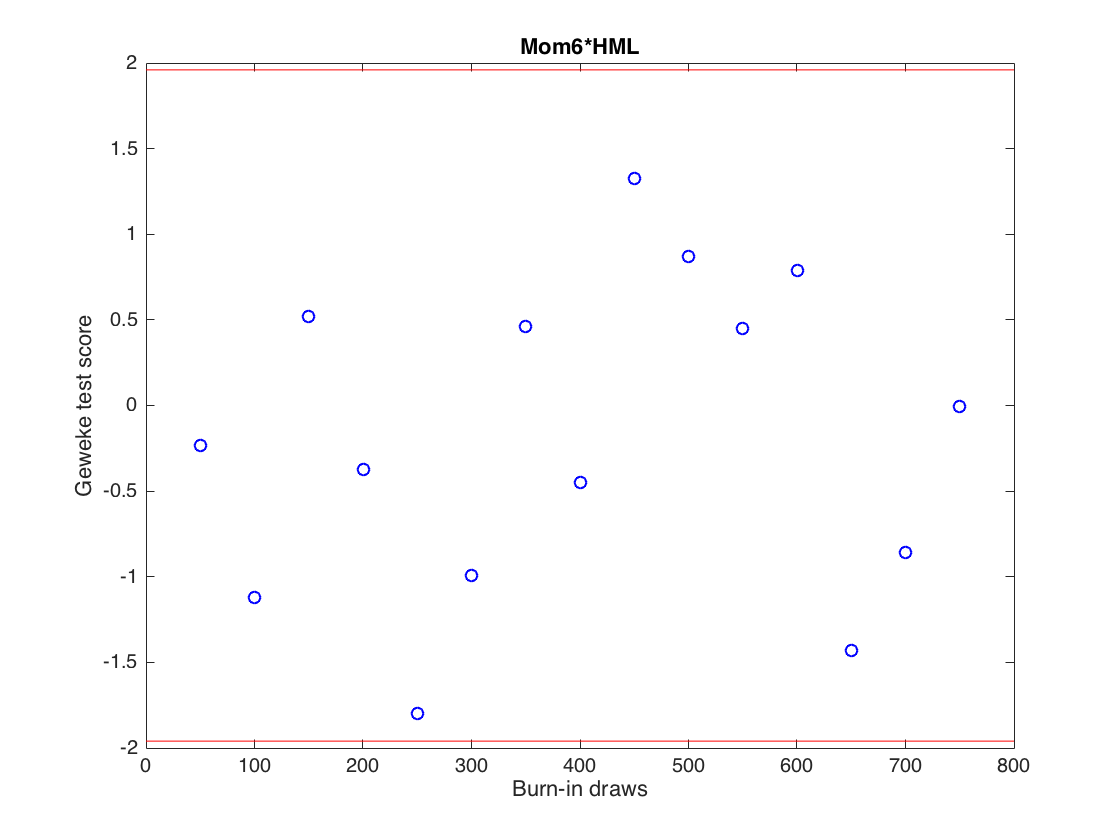
\includegraphics[width = 9cm, height = 7.5cm]{pictures/geweke1.png}
 
%     \end{subfigure}%
%     ~ 
%     \begin{subfigure}[b]{0.5\textwidth}
%         \centering
% \captionsetup{justification=centering,font=small,labelfont=footnotesize}
  
%         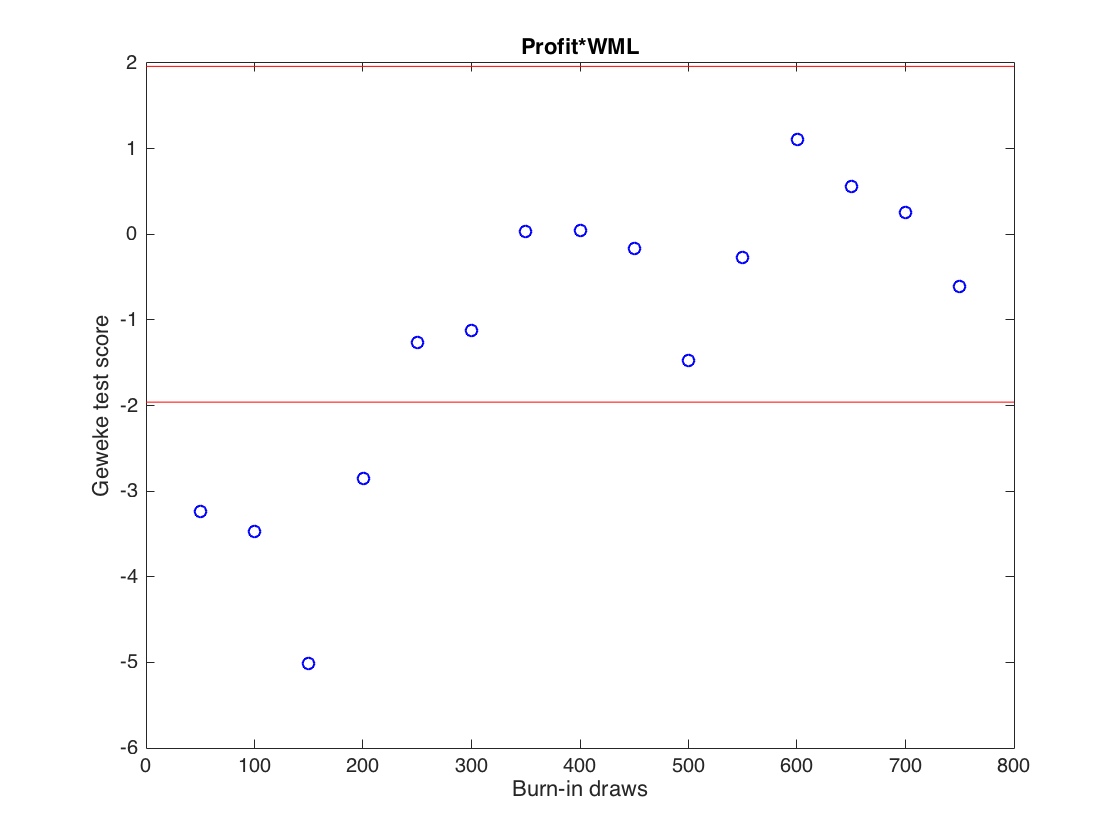
\includegraphics[width = 9cm, height = 7.5cm]{pictures/geweke2.png}
        
        

%     \end{subfigure}
    
%         \begin{subfigure}[b]{0.5\textwidth}
%         \centering 
%               \captionsetup{justification=centering, font=small,labelfont=footnotesize}
%         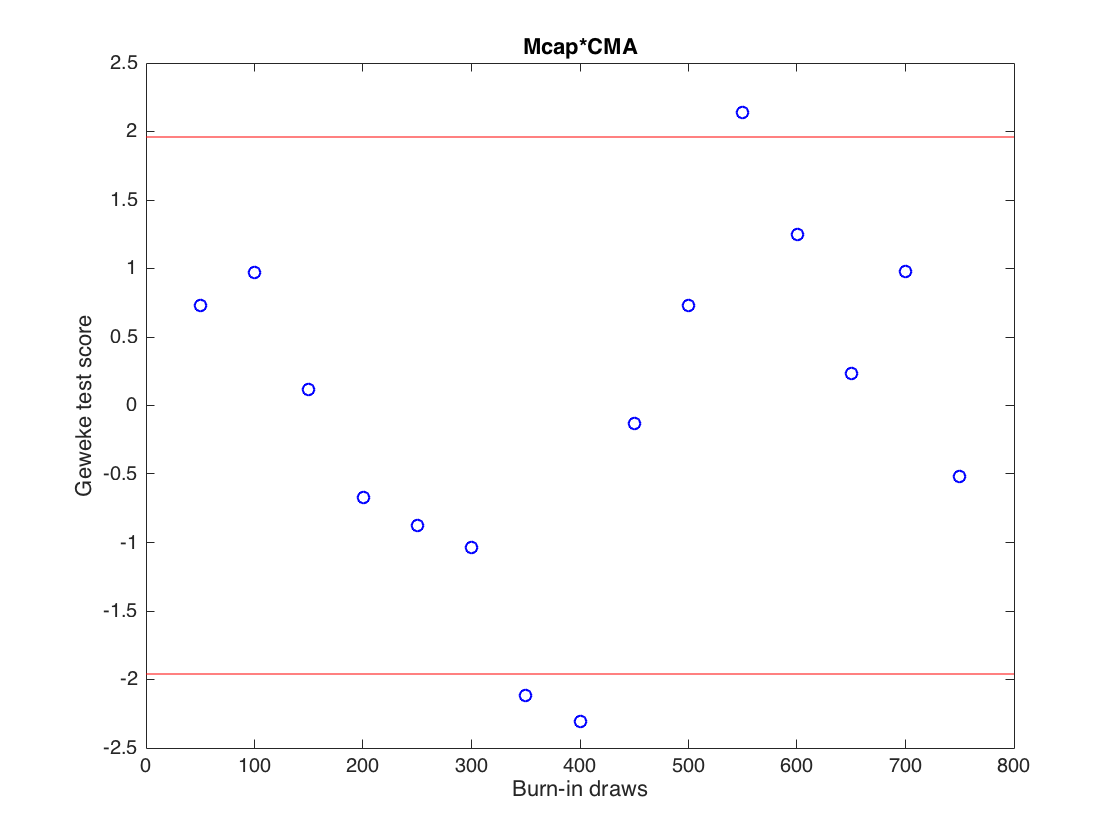
\includegraphics[width = 9cm, height = 7.5cm]{pictures/geweke3.png}
 
%     \end{subfigure}%
%     ~ 
%     \begin{subfigure}[b]{0.5\textwidth}
%         \centering
% \captionsetup{justification=centering,font=small,labelfont=footnotesize}
  
%         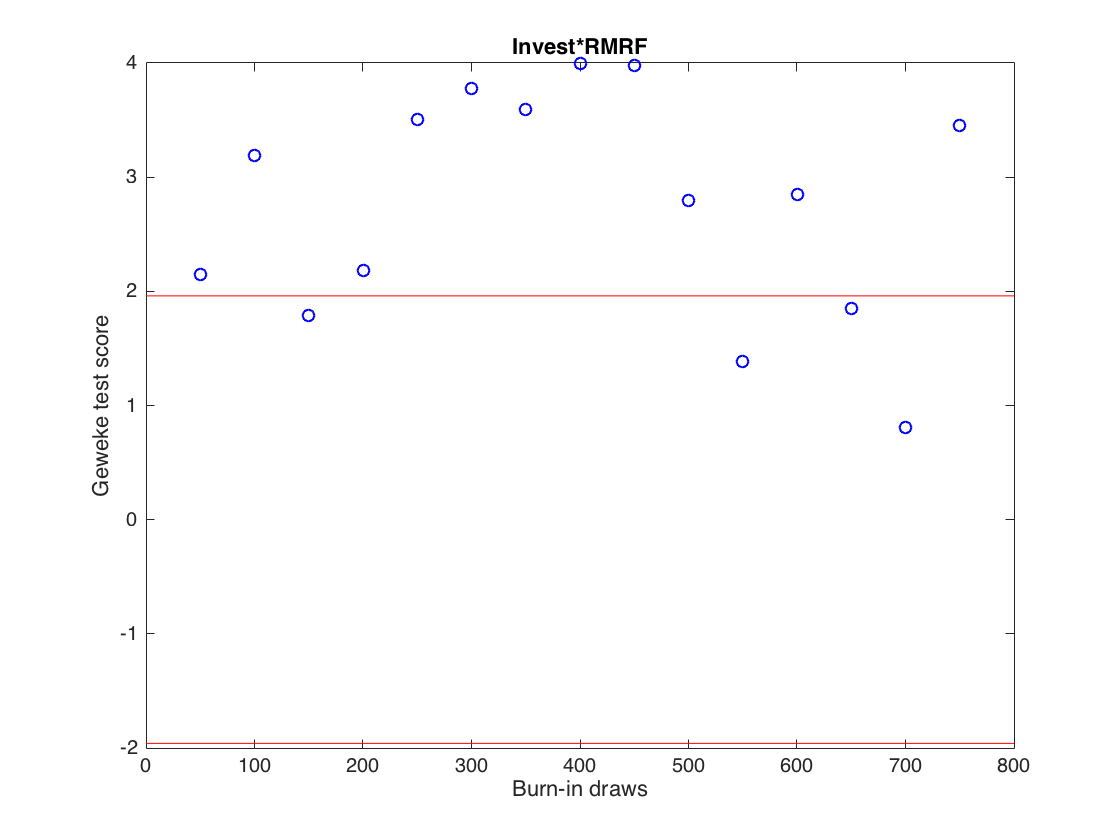
\includegraphics[width = 9cm, height = 7.5cm]{pictures/geweke4.png}
%             \end{subfigure}

% \end{figure}

% \subsubsection*{Derivation of full conditional posterior distributions}
% We provide the derivation of the full conditional posterior distributions of the parameters. The joint posterior distribution is written as 
% \begin{equation}
%     \label{posterior}
%     p(\Theta|R) \propto p(\Theta)p(R|\Theta).
% \end{equation}
% We can write the likelihood function of the data, $p(R|\Theta)$, as 
% \begin{equation}
%     p(R|\Theta) \propto \prod_{i=1}^{N} \frac{1}{\sigma^{T_i}_{\eta_i}} \text{exp}\left(-\frac{1}{2\sigma^2_{\eta_i}}(R_i-G_i\theta_i - H_i\xi)' (R_i-G_i\theta_i - H_i\xi)\right). 
% \end{equation}
%  We partition the set of model parameters $\Theta$ into separate blocks and derive the full conditional posterior distribution for each block. To derive the full conditional posterior for block $d$, that is, $d|\Theta_{-d},R$ with $\Theta_{-d}$ containing all parameters in $\Theta$ except $d$, we simply need to collect all the terms in $p(\Theta|R)$ depending on $d$. 
%  \par Regarding the fund-specific parameters $\theta_i$, we group all the terms in $p(\Theta|R)$ depending on $\theta_i$, such that we can derive the full conditional posterior distribution using the following steps


% \begin{alignat}{2}
% \label{proof1}
% p(\theta_i|\Theta_{-\theta_i},R) &\propto p(\theta_i)p(R|\Theta)  \nonumber  \\
%  &\propto \text{exp}\left(-\frac{1}{2}(\theta_i-\bar{\theta})'\Sigma^{-1}_{\theta} (\theta_i-\bar{\theta})\right) \text{exp}\left(-\frac{1}{2\sigma^2_{\eta_i}}(R_i-G_i\theta_i - H_i\xi)' (R_i-G_i\theta_i - H_i\xi)\right) \nonumber  \\ 
%       &= \text{exp}\left(-\frac{1}{2}\left[(\theta_i-\bar{\theta})'\Sigma^{-1}_{\theta} (\theta_i-\bar{\theta}) + \frac{1}{\sigma^2_{\eta_i}}(Y_i-G_i\theta_i)' (Y_i-G_i\theta_i )\right]\right)    \justif{\quad}{\text{Let} \hspace{0.1cm} 
%             Y_i = R_i - H_i\xi} \nonumber  \\ 
%              &= \text{exp}\left(-\frac{1}{2}\left[(\Sigma^{-\frac{1}{2}}_{\theta}\bar{\theta} - \Sigma^{-\frac{1}{2}}_{\theta} \theta_i)'(\Sigma^{-\frac{1}{2}}_{\theta}\bar{\theta} - \Sigma^{-\frac{1}{2}}_{\theta} \theta_i) + \frac{1}{\sigma^2_{\eta_i}}(Y_i-G_i\theta_i)' (Y_i-G_i\theta_i )\right]\right)                  \justif{\quad}{\text{Use} \hspace{0.1cm} [1]} \nonumber  \\
%   &=  \text{exp}\left(-\frac{1}{2}(w_i-V_i\theta_i)' (w_i-V_i\theta_i)\right)   \justif{\quad}{\text{Let} \hspace{0.15cm} w_i = \left[\frac{Y_i}{\sigma_{\eta_i}} \hspace{0.25cm} \Sigma^{-\frac{1}{2}}_{\theta}\bar{\theta} \right]' \hspace{0.15cm} \text{and} \hspace{0.15cm} V_i =  \left[\frac{G_i}{\sigma_{\eta_i}} \hspace{0.25cm} \Sigma^{-\frac{1}{2}}_{\theta} \right]'   } \nonumber   \\
%  &\propto \text{exp}\left(-\frac{1}{2}(\theta_i -\hat{\theta}_i)' V_i'V_i(\theta_i -\hat{\theta}_i)\right)     \justif{\quad}{\text{Use} \hspace{0.1cm} [2], \hspace{0.1cm} \text{with} \hspace{0.15cm} \hat{\theta}_i = (V_i'V_i)^{-1} V_iw_i, } \nonumber \\
% \end{alignat} 
% which is the kernel of a multivariate normal distribution, that is, the full conditional posterior distribution of $\theta_i$  is given by

% \begin{equation}
%     \theta_i|\Theta_{-\theta_i},R \sim \mathcal{N}\left(\tilde{\theta}_i,\tilde{\Sigma}_{\theta_i}\right), 
% \end{equation}
% with parameters
% \begin{equation}
%     \tilde{\theta}_i = \hat{\theta}_i = \tilde{\Sigma}_{\theta_i}\left(\frac{1}{\sigma^{2}_{\eta_i}}G_i'(R_i - H_i\xi) + \Sigma^{-1}_{\theta}\bar{\theta} \right) 
% \end{equation}
% \begin{equation}
%     \tilde{\Sigma}_{\theta_i} =  (V_i'V_i)^{-1} =\left(\frac{1}{\sigma^2_{\eta_i}}G_i'G_i +  \Sigma^{-1}_{\theta}\right)^{-1}. 
% \end{equation}
% Using the same steps as in \ref{proof1}, the full conditional posterior of $\bar{\theta}$ is given by 

%     \begin{equation}
%     \bar{\theta}|\Theta_{-\bar{\theta}},R \sim \mathcal{N}\left(\tilde{\bar{\theta}},\tilde{\Sigma}_{\bar{\theta}}\right),
% \end{equation}
% with parameters
% \begin{equation}
%     \tilde{\bar{\theta}} = \tilde{\Sigma}_{\bar{\theta}}\left(\Sigma^{-1}_{\theta} \sum^N_{i = 1} \theta_i + \Sigma^{-1}_{\mathit{k}} \mathit{k}\right) 
% \end{equation}
% \begin{equation}
%     \tilde{\Sigma}_{\bar{\theta}} =  \left(N \Sigma^{-1}_{\theta} +  \Sigma^{-1}_{\mathit{k}}\right)^{-1}. 
% \end{equation}

% \blfootnote{[1] Choleski decomposition: $B^{-1}$ = $B^{-\frac{1'}{2}}$$B^{-\frac{1}{2}}$.}
% \blfootnote{[2] Decomposition rule: $(y-X\beta)'(y-X\beta)$ = $(y-X\hat{\beta})'(y-X\hat{\beta})$ + $(\beta - \hat{\beta})'X'X(\beta - \hat{\beta})$,  where $\hat{\beta}$ = $(X'X)^{-1}X'y$. }
% \blfootnote{[3] Product of determinants: $|A||B|$ = $|AB|$.}
% \blfootnote{[4] Trace of a scalar: $A$ = Tr($A$), where $A$ is a scalar.}
% \blfootnote{[5] Invariance of the trace under cyclic permutations: Tr$(ABC)$ = Tr($CAB$) = Tr($BCA$).}
% \blfootnote{[6] Sum of traces: Tr($A$) + Tr($B$) = Tr($A$+$B$).}

% \noindent Regarding the covariance matrix $\Sigma_{\theta}$, we derive the full conditional posterior as follows

% \begin{alignat}{2}
% p(\Sigma_{\theta}|\Theta_{-\Sigma_{\theta}},R) &\propto p(\Sigma_{\theta}) \prod^N_{i=1}p(\theta_i)  \nonumber  \\
%  &\propto |\Sigma_{\theta}|^{-\frac{\psi_{\theta} + k + 1}{2}}  \text{exp}\left(-\frac{1}{2}\text{tr}(\Sigma^{-1}_{\theta} \psi_{\theta}S_{\theta})\right) \prod^N_{i=1} |\Sigma_{\theta}|^{-\frac{1}{2}}  \text{exp}\left(-\frac{1}{2}(\theta_i - \bar{\theta})' \Sigma^{-1}_{\theta}(\theta_i - \bar{\theta})\right) \nonumber  \\ 
%       &= 
%       |\Sigma_{\theta}|^{-\frac{\psi_{\theta} + N+k + 1}{2}} \text{exp}\left(-\frac{1}{2}\left[\text{tr}(\Sigma^{-1}_{\theta} \psi_{\theta}S_{\theta}) + \text{tr}\left(\sum^N_{i=1}(\theta_i - \bar{\theta})' \Sigma^{-1}_{\theta}(\theta_i - \bar{\theta}) \right) \right]\right)    \justif{\quad}{\text{Use}\hspace{0.1cm} [3]+[4]} \nonumber  \\ 
% &= 
%       |\Sigma_{\theta}|^{-\frac{\psi_{\theta} + N+k + 1}{2}} \text{exp}\left(-\frac{1}{2}\left[\text{tr}( \Sigma^{-1}_{\theta} \psi_{\theta}S_{\theta}) + \text{tr}\left(\sum^N_{i=1}\Sigma^{-1}_{\theta}(\theta_i - \bar{\theta})(\theta_i - \bar{\theta})' \right) \right]\right)    \justif{\quad}{\text{Use}\hspace{0.1cm} [5]} \nonumber  \\ 
% &= 
%       |\Sigma_{\theta}|^{-\frac{\psi_{\theta} + N+k + 1}{2}} \text{exp}\left(-\frac{1}{2}\text{tr}\left(  \Sigma^{-1}_{\theta} \left[\sum^N_{i=1}(\theta_i - \bar{\theta}) (\theta_i - \bar{\theta})' +  \psi_{\theta}S_{\theta} \right]\right)\right)    \justif{\quad}{\text{Use}\hspace{0.1cm} [6]}, \nonumber  \\ 
% \end{alignat} 
% which is the kernel of an inverted Wishart distribution, that is, the full conditional posterior distribution of $\Sigma_{\theta}$ is given by 
% \begin{equation}
%     \Sigma_{\theta}|\Theta_{-\Sigma_{\theta}},R \sim \mathit{IW}\left(\sum^N_{i=1}(\theta_i-\bar{\theta})(\theta_i-\bar{\theta})'+\psi_{\theta}S_{\theta},\psi_{\theta} + N\right)
% \end{equation}
% Using the same steps as in \ref{proof1}, the full conditional posterior of $\xi$ is given by
% \begin{equation}
%     \xi|\Theta_{-\xi} \sim \mathcal{N}(\tilde{\xi},\tilde{\Sigma}_{\xi}),
% \end{equation}
% with parameters 

% \begin{equation}
%     \tilde{\xi} = \tilde{\Sigma}_{\xi}\left(\sum^N_{i=1}\frac{1}{\sigma^2_{\eta_i}} H_i'(R_i - G_i\theta_i) + \Sigma^{-1}_{\xi} \bar{\xi}\right) 
% \end{equation}

% \begin{equation}
%     \tilde{\Sigma}_{\xi} =  \left(\sum^N_{i=1}\frac{1}{\sigma^2_{\eta_i}}  H_i'H_i + \Sigma^{-1}_{\xi}\right)^{-1}. 
% \end{equation}
% Finally, we derive the full conditional posterior of $\sigma^2_{\eta_i}$ as follows 

% \begin{alignat}{2}
% p(\sigma^2_{\eta_i}|\Theta_{-\Sigma_{\sigma^2_{\eta_i}}},R) &\propto p(\sigma^2_{\eta_i})p(R|\Theta)  \nonumber  \\
%  &\propto \sigma^{-(T_i+2)}_{\eta_i}  \text{exp}\left(-\frac{1}{2\sigma^2_{\eta_i}}(R_i - G_i\theta_i -H_i\xi)'(R_i - G_i\theta_i -H_i\xi)\right), \nonumber  \\ 
% \end{alignat} 
% which is the kernel of an inverted Gamma-2 distribution, that is, the full conditional posterior distribution of $\sigma^2_{\eta_i}$ is given by 
% \begin{equation}
%     \sigma^2_{\eta_i}|\Theta_{-\sigma^2_{\eta_i}} \sim \mathit{IG}2\left((R_i - G_i\theta_i -H_i\xi)'(R_i - G_i\theta_i -H_i\xi),T_i\right).
% \end{equation}
% \begin{table}[H]
% \centering
% \small
% \centering
% \setlength{\tabcolsep}{21pt}
% {\captionsetup{justification=centering,singlelinecheck=off}
% \caption*{\bfseries Table A2: Four-factor model alpha vs fund-level charactersistics }}
% \caption*{This table presents the time-series averages of coefficients ($c$) from monthly regressions,
% \begin{equation*}
% \label{a}
%     \alpha_{it} = c_{0t} + c_{1t}Z_{it-1} + u_i.
% \end{equation*}
% We employ the \citet{carhart1997persistence} four-factor model. The alphas ($\alpha_{it})$ are estimated with OLS from rolling time series using returns from time $t$-35 until $t$. The fund characteristics (Z) are the logarithm of the market capitalization (Mcap), the logarithm of the book-to-market ratio (B/M), and the logarithm of one plus the cumulative past six-month cumulative return (Mom6). We calculate fund-level characteristics by a portfolio-weighted average across individual fund holdings. Each fund-level characteristic is winsorized at the 0.5\% and the 99.5\% levels. We also standardize each fund-level characteristic by subtracting its monthly cross-sectional mean. Panel A reports average four-factor alphas in quintiles sorted on characteristics. T-statistics with the \citet{newey1986simple} correction of 12 lags are in parenthesis. Significant alphas at the 5\% level are in bold font. Panel B reports the average coefficients from the monthly regressions. \citet{fama1973risk} t-statistics with the \citet{newey1986simple} correction of 12 lags are in parenthesis. Estimates significant at the 5\% level are in bold font. The sample period is April 1983 to December 2015.   }
% {\captionsetup{justification=centering,singlelinecheck=off}
% \caption*{Panel A: Average four-factor alpha in quintiles sorted on characteristics  }
% \begin{tabular}{crrr}
% \hline
% Quintile & \multicolumn{1}{c}{Mcap} & \multicolumn{1}{c}{B/M} & \multicolumn{1}{c}{Mom6} \\ \hline
% 1        & -0.044                   & -0.015                  & \textbf{-0.065}          \\
%          & (-1.49)                  & (-0.51)                 & (-3.10)                  \\
% 2        & 0.001                    & -0.048                  & -0.045                   \\
%          & (0.02)                   & \textbf{(-2.06)}        & \textbf{(-2.81)}         \\
% 3        & -0.037                   & -0.041                  & -0.038                   \\
%          & (1.85)                   & (-2.21)                 & (-2.13)                  \\
% 4        & \textbf{-0.059}          & \textbf{-0.049}         & -0.035                   \\
%          & (-4.06)                  & (-2.70)                 & (-1.66)                  \\
% 5        & \textbf{-0.074}          & \textbf{-0.060}         & -0.020                   \\
%          & (-6.39)                  & (-2.64)                 & (-0.78)                  \\
% 5-1      & -0.030                   & -0.045                  & \textbf{0.045}           \\
%          & (-1.09)                  & (-1.36)                 & (2.34)                   \\ \hline
% \end{tabular}
% \end{table}

% \begin{table}[H]
% \centering
% \small
% \setlength{\tabcolsep}{15.5pt}
% {\captionsetup{justification=centering,singlelinecheck=off}
% \caption*{ Panel B: Cross-sectional regressions of four-factor alpha on characteristics }}
% \begin{tabular}{crrrr}
% \hline
% Cnt  & \textbf{-0.042} & \textbf{-0.042} & \textbf{-0.042} & \textbf{-0.042} \\ \hline
%      & (-2.20)         & (-2.20)         & (-2.20)         & (-2.20)         \\
% Mcap & -0.003          &                 &                 & -0.002          \\
%      & (-1.77)         &                 &                 & (-1.14)         \\
% B/M  &                 & -0.049          &                 & -0.023          \\
%      &                 & (-0.72)         &                 & (-0.36)         \\
% Mom6 &                 &                 & \textbf{0.003}  & 0.001           \\
%      &                 &                 & (2.03)          & (1.26)          \\ \hline
% \end{tabular}
% \end{table}


% \begin{table}[H]
% \centering
% \small
% \centering
% \setlength{\tabcolsep}{24pt}
% {\captionsetup{justification=centering,singlelinecheck=off}
% \caption*{\bfseries Table A3: DGTW characteristic selectivity measure vs four-factor fund betas}}
% \caption*{This table presents the time-series averages of coefficients ($c$) from monthly regressions,
% \begin{equation*}
% \label{a}
%     \text{DGTW}_{i,t-35:t} = c_{0t} + c_{1t}\hat{B}_{it} + u_i.
% \end{equation*}
% We employ the characteristic selectivity (CS) measure of Daniel, Grinblatt, Titman, and Wermens (DGTW; 1997). The dependent variable $\text{DGTW}_{i,t-35:t}$ is the time series average of the DGTW CS measure over the period from time $t$-35 until $t$. Using fund returns over this period, we estimate the factor betas ($\hat{B}_{it}$) from the four-factor model of \citet{carhart1997persistence}. We standardize each factor beta by subtracting its monthly cross-sectional mean. Panel A reports the average DGTW CS measure in quintiles sorted on factor betas. T-statistics with the \citet{newey1986simple} correction of 12 lags are in parenthesis. Significant DGTW CS measures at the 5\% level are in bold font. Panel B reports the average coefficients from the monthly regressions. \citet{fama1973risk} t-statistics with the \citet{newey1986simple} correction of 12 lags are in parenthesis. Estimates significant at the 5\% level are in bold font. The sample period is April 1983 to December 2015.  }
% {\captionsetup{justification=centering,singlelinecheck=off}
% \caption*{Panel A: Average DGTW CS measure in quintiles sorted on four-factor betas  }
% \begin{tabular}{crrr}
% \hline
% Quintile & SMB            & HML            & WML             \\ \hline
% 1        & \textbf{0.021} & 0.038          & \textbf{-0.049} \\
%          & (2.26)         & (1.38)         & (-3.16)         \\
% 2        & 0.004          & 0.014          & 0.005           \\
%          & (0.47)         & (1.31)         & (0.44)          \\
% 3        & \textbf{0.025} & \textbf{0.025} & \textbf{0.028}  \\
%          & (2.39)         & (2.93)         & (3.42)          \\
% 4        & \textbf{0.049} & \textbf{0.028} & \textbf{0.053}  \\
%          & (4.58)         & (2.13)         & (6.76)          \\
% 5        & 0.053          & 0.028          & \textbf{0.096}  \\
%          & (1.91)         & (1.47)         & (5.46)          \\
% 5-1      & 0.032          & -0.053         & \textbf{0.052}  \\
%          & (1.74)         & (-0.23)        & (6.33)          \\ \hline
% \end{tabular}
% \end{table}

% \begin{table}[H]
% \centering
% \small
% \setlength{\tabcolsep}{12pt}
% {\captionsetup{justification=centering,singlelinecheck=off}
% \caption*{ Panel B: Cross-sectional regressions of DGTW CS measure on four-factor betas}}
% \label{my-label}
% \begin{tabular}{crrrrr}
% \hline
% Cnt  & \textbf{0.027} & \textbf{0.027} & \textbf{0.027} & \textbf{0.027} & \textbf{0.027} \\
%      & (3.25)         & (3.25)         & (3.25)         & (3.25)         & (3.25)         \\
% RMRF & -0.031         &                &                &                & -0.073         \\
%      & (-0.50)        &                &                &                & (-1.42)        \\
% SMB  &                & 0.067          &                &                & 0.036          \\
%      &                & (1.93)         &                &                & (1.64)         \\
% HML  &                &                & -0.002         &                & 0.003          \\
%      &                &                & (-0.04)        &                & (0.07)         \\
% WML  &                &                &                & \textbf{0.364} & \textbf{0.347} \\
%      &                &                &                & (7.73)         & (10.17)        \\ \hline
% \end{tabular}
% \end{table}

% \begin{table}[H]
% \small
% {\captionsetup{justification=centering,singlelinecheck=off}
% \caption*{\bfseries Table A2: Mutual Fund Performance Persistence }}
% \caption*{This table presents returns of decile porfolios sorted by the \citet{carhart1997persistence} four-factor model alpha (Panel A), double-adjusted four-factor alpha (Panel B) and characteristic-driven performance (Panel C). These performance measured are calculated using rolling windows with a window size of 36 months. Portfolios are rebalanced every quarter-end and are held for up to six years. To deal with overlapping portfolios, we follow \citet{jegadeesh1993returns} to take the equal-weighted return across overlapping portfolios formed in different quarters. Two different returns are reported: the excess return over the risk-free rate and the four-factor alpha. T-statistics, shown in parenthesis, are computed using White's standard errors. Estimated significant at the 5\% level are in bold font. The sample period is May 1980 to December 2015.}
% \label{my-label}
% \begin{tabular}{cccccccccccc}
% \hline
%       & \multicolumn{2}{c}{Qtr 1} &  & \multicolumn{2}{c}{Qtr 1-4} &  & \multicolumn{2}{c}{Qtr 5-12} &  & \multicolumn{2}{c}{Qtr 13-24} \\ \cline{2-3} \cline{5-6} \cline{8-9} \cline{11-12} 
% Decile & Excess     & 4F alpha     &  & Excess      & 4F alpha      &  & Excess       & 4F alpha      &  & Excess       & 4F alpha       \\ \hline
% \multicolumn{12}{l}{Panel A: Carhart four-factor alpha}                                                                                          \\
% 1      & 0.52       & -0.16        &  & 0.56        & -0.15         &  & 0.56         & -0.14         &  & 0.48         & -0.15          \\
% 2      & 0.55       & -0.09        &  & 0.54        & -0.12         &  & 0.55         & -0.10         &  & 0.52         & -0.09          \\
% 3      & 0.56       & -0.08        &  & 0.55        & -0.09         &  & 0.56         & -0.08         &  & 0.55         & -0.07          \\
% 4      & 0.53       & -0.10        &  & 0.56        & -0.08         &  & 0.55         & -0.08         &  & 0.53         & -0.08          \\
% 5      & 0.58       & -0.07        &  & 0.57        & -0.07         &  & 0.55         & -0.09         &  & 0.50         & -0.11          \\
% 6      & 0.57       & -0.07        &  & 0.58        & -0.06         &  & 0.54         & -0.09         &  & 0.53         & -0.08          \\
% 7      & 0.60       & -0.04        &  & 0.58        & -0.05         &  & 0.55         & -0.06         &  & 0.53         & -0.08          \\
% 8      & 0.59       & -0.05        &  & 0.60        & -0.03         &  & 0.56         & -0.05         &  & 0.52         & -0.08          \\
% 9      & 0.62       & -0.02        &  & 0.61        & -0.02         &  & 0.55         & -0.06         &  & 0.53         & -0.08          \\
% 10     & 0.71       & 0.03         &  & 0.66        & 0.01          &  & 0.60         & -0.03         &  & 0.57         & -0.07          \\
% 10-1  & 0.19       & 0.20         &  & 0.11        & 0.16          &  & 0.04         & 0.11          &  & 0.09         & 0.08           \\
%       & (\bf{3.47})       & (\bf{3.49})         &  & (\bf{2.32})        & (\bf{3.21})         &  & (\bf{0.73})         & (\bf{2.01})          &  & (1.69)         & (1.73)           \\
%       &            &              &  &             &               &  &              &               &  &              &                \\
% \multicolumn{12}{l}{Panel B: Double-adjusted Carhart four-factor alpha}                                                                          \\
% 1      & 0.56       & -0.14        &  & 0.57        & -0.14         &  & 0.54         & -0.14         &  & 0.47         & -0.16          \\
% 2      & 0.56       & -0.08        &  & 0.56        & -0.10         &  & 0.55         & -0.10         &  & 0.53         & -0.09          \\
% 3      & 0.54       & -0.11        &  & 0.57        & -0.09         &  & 0.56         & -0.09         &  & 0.53         & -0.09          \\
% 4      & 0.57       & -0.07        &  & 0.58        & -0.07         &  & 0.55         & -0.09         &  & 0.52         & -0.09          \\
% 5      & 0.59       & -0.05        &  & 0.56        & -0.07         &  & 0.54         & -0.09         &  & 0.52         & -0.09          \\
% 6      & 0.57       & -0.07        &  & 0.57        & -0.06         &  & 0.55         & -0.07         &  & 0.52         & -0.08          \\
% 7      & 0.58       & -0.05        &  & 0.57        & -0.06         &  & 0.55         & -0.06         &  & 0.53         & -0.08          \\
% 8      & 0.57       & -0.07        &  & 0.59        & -0.04         &  & 0.55         & -0.06         &  & 0.51         & -0.09          \\
% 9      & 0.63       & -0.01        &  & 0.61        & -0.03         &  & 0.57         & -0.04         &  & 0.55         & -0.06          \\
% 10     & 0.67       & 0.01         &  & 0.64        & -0.01         &  & 0.59         & -0.04         &  & 0.57         & -0.06          \\
% 10-1  & 0.11       & 0.15         &  & 0.07        & 0.13          &  & 0.05         & 0.11          &  & 0.10         & 0.10           \\
%       & (\textbf{3.10})       & (\textbf{4.13})         &  & (\textbf{2.39})        & (\textbf{4.23})          &  & (1.34)         & (\textbf{2.94})          &  & (\textbf{2.56})         & (\textbf{3.31})           \\
%       &            &              &  &             &               &  &              &               &  &              &                \\
% \multicolumn{12}{l}{Panel C: Characteristic-driven performance}                                                                       \\
% 1      & 0.49       & -0.11        &  & 0.54        & -0.11         &  & 0.61         & -0.06         &  & 0.53         & -0.09          \\
% 2      & 0.53       & -0.08        &  & 0.57        & -0.07         &  & 0.60         & -0.05         &  & 0.54         & -0.07          \\
% 3      & 0.53       & -0.09        &  & 0.56        & -0.08         &  & 0.57         & -0.07         &  & 0.54         & -0.06          \\
% 4      & 0.55       & -0.07        &  & 0.57        & -0.06         &  & 0.56         & -0.08         &  & 0.52         & -0.08          \\
% 5      & 0.57       & -0.06        &  & 0.59        & -0.04         &  & 0.56         & -0.07         &  & 0.54         & -0.07          \\
% 6      & 0.60       & -0.06        &  & 0.60        & -0.06         &  & 0.55         & -0.08         &  & 0.52         & -0.09          \\
% 7      & 0.62       & -0.06        &  & 0.58        & -0.08         &  & 0.54         & -0.10         &  & 0.52         & -0.10          \\
% 8      & 0.62       & -0.05        &  & 0.59        & -0.06         &  & 0.53         & -0.10         &  & 0.52         & -0.10          \\
% 9      & 0.64       & -0.03        &  & 0.60        & -0.06         &  & 0.52         & -0.09         &  & 0.51         & -0.11          \\
% 10     & 0.70       & -0.02        &  & 0.61        & -0.06         &  & 0.53         & -0.08         &  & 0.54         & -0.10          \\
% 10-1  & 0.20       & 0.10         &  & 0.06        & 0.06          &  & -0.09        & -0.01         &  & 0.01         & -0.01          \\
%       & (1.58)       & (0.80)         &  & (0.61)        & (0.60)         &  & (-0.89)        & (-0.14)         &  & (0.15)         & (-0.12)          \\ \hline
% \end{tabular}
% \end{table}
